\chapter{Results}

In this chapter, we analyze the performance of our software and compare its results to those of the Tesseract \textsc{TableFind} algorithm. For these purposes, we use our own testing set of over 160 images containing one or more tables. We deliberately chose images that are not scanned or disrupted in any way, as this might negatively affect the results of Tesseract recognition, which both our implementation and Tesseract's TableFind rely on.

\section{Performance measurements}

As already mentioned, Tesseract is an engine heavy on resources. Its recognition and its functions therefore take a great amount of time, which is also the reason why the time complexity of our implementation is significantly higher.

For comparison, when we run our software on a single image ($1654\times2339$, of size 675~KB), the absolute time of recognition is 11.6~seconds. Tesseract's API initialization takes 9.6~seconds of this time (with its \texttt{recognize} function performing the character and line recognition in 9.2~seconds), and our functions for saving results (which use the calls of Leptonica) take 0.5~seconds. About 1.4~seconds is consumed by our \texttt{init\_textlines} function, which also uses the calls of the Tesseract API. However, this function needs to iterate over all symbols and textlines multiple times, which also adds to the time complexity. The time complexity of the other functions (which is below 0.1~seconds) is therefore negligible.

We ran a performance test on all our images to provide a better concept of the amount of time that our software spends on each function. We did not add any preprocessing, as it is a part of the Leptonica library and therefore does not affect the performance of entirely our functions. Furthermore, upon running a few tests on the preprocessor functions, they seemed to barely affect the performance.

The results were as follows: the calls of Tesseract API took 65.94\% of the overall time, our textline initialization 30.26\%, result saving 2.9\% and the other functions solely 0.9\%. However, despite these results, we have observed that time complexity of the textline initialization does not exceed 20\% in most cases. However, a few images, usually those containing full-page tables, spend even more time analyzing textlines than with the actual recognition, which significantly affects the overall results.

In the following sections, we will discuss the options of reducing this time complexity in favor of the results accuracy. This includes the discussion about the effects of the quality of an image on the results and time complexity, as well as the effects of the amount of text in an image on the time complexity.

\section{Effects of the amount of text} \label{resultsEffectsOfText}

In this section, we provide an overview of the effects of the number of recognized symbols and textlines on the execution time of our algorithm. As we already mentioned in~\cref{textlineInitialization}, the time complexity of our \texttt{init\_textlines} function is $O(m*n^2)$ (where m represents the amount of textlines and n the amount of symbols). Therefore, the greater the amount of textlines and symbols, the more time this function will consume. However, the time complexity of the Tesseract recognition also greatly depends on the amount of textlines and symbols it eventually finds. We tested these dependencies on a subset of 18 of the already mentioned images. We presented all of them in various (about 15) different resolutions, ranging from 25 to 800 dpi, to our recognition system. 

This gave us a reasonably diverse set of different images. We used the results from the tests to present the mentioned dependencies in \cref{fig:symbolsTimeInit,fig:symbolsTimeTess,fig:symbolsTime,fig:textlinesTimeInit,fig:textlinesTimeTess,fig:textlinesTime}.

By observing the testing results and utilizing the above mentioned graphs, we may conclude the following statements:

\begin{itemize}
    \item \emph{For our table detection algorithm to detect a table, Tesseract needs to recognize above 800 symbols and 40 textlines.}
    
    If our algorithm is presented with either smaller amount of symbols or textlines, then either the Tesseract recognition system failed to recognize most of the page content, or the page has so little text information that there is almost no chance of it representing a table. Our table detection algorithm is therefore presumed to fail.

    \item \emph{The time of the execution of our \texttt{init\_textlines} function grows with the number of symbols and textlines.}
    
    As already expected, the time complexity of this function grows exponentially in both the textline and symbol case. We present this dependency in~\cref{fig:symbolsTimeInit} and~\cref{fig:textlinesTimeInit}.

    \item \emph{The time of the Tesseract recognition greatly depends on the number of symbols, not so much on textlines.}
    
    The recognition of symbols and textlines is performed concurrently~\cref{tesseractCharacterRecognition}. However, what Tesseract focuses on during this process is the merging and recognition of the individual characters, while the textlines are only a side product. Therefore, the dependencies in graph~\cref{fig:textlinesTimeTess} could be completely different and the graph does not contain any meaningful information.
    
\end{itemize}

\begin{figure}[t]
\minipage{0.45\textwidth}
    \centering
    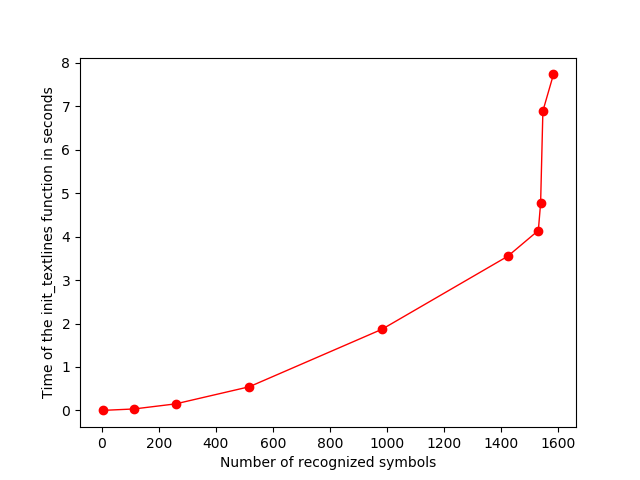
\includegraphics[width=\linewidth]{img/results/symbolsTimeInit.png}
    \caption{The time of execution of the \texttt{init\_textlines} function with respect to the number of recognized textlines.}
    \label{fig:symbolsTimeInit}
\endminipage\hfill
\minipage{0.45\textwidth}
    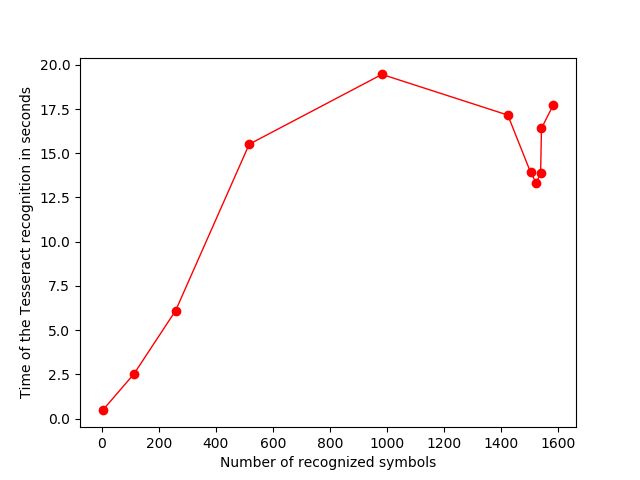
\includegraphics[width=\linewidth]{img/results/symbolsTimeTesseract.png}
    \caption{The time of execution of Tesseract recognition with respect to the number of recognized textlines.}
    \label{fig:symbolsTimeTess}
\endminipage\\
\minipage{0.45\textwidth}
    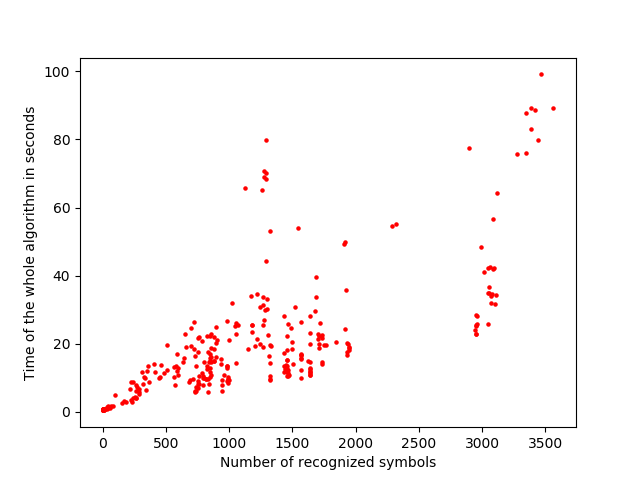
\includegraphics[width=\linewidth]{img/results/symbolsTimeAll.png}
    \caption{The overall time of execution with respect to the number of recognized symbols.}
    \label{fig:symbolsTime}
\endminipage\hfill 
\minipage{0.45\textwidth}
    \centering
    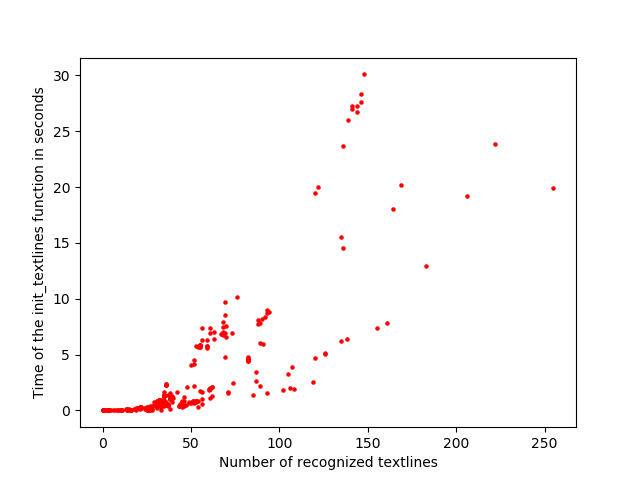
\includegraphics[width=\linewidth]{img/results/textlinesTimeInit.png}
    \caption{The time of execution of the \texttt{init\_textlines} function with respect to the number of recognized textlines.}
    \label{fig:textlinesTimeInit}
\endminipage\\
\minipage{0.45\textwidth}
    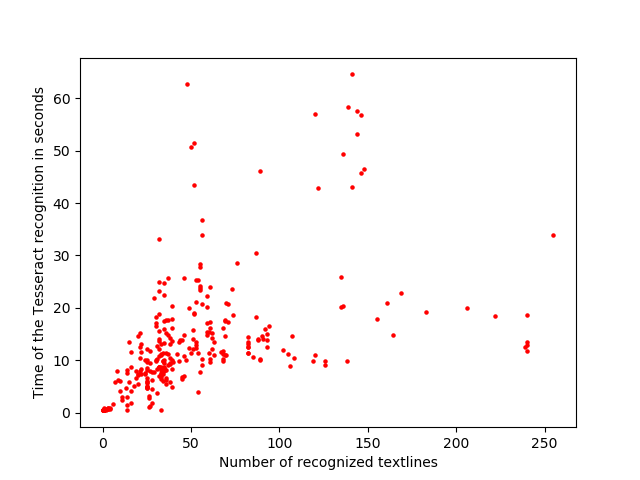
\includegraphics[width=\linewidth]{img/results/textlinesTimeTesseract.png}
    \caption{The time of execution of Tesseract recognition with respect to the number of recognized textlines.}
    \label{fig:textlinesTimeTess}
\endminipage\hfill
\minipage{0.45\textwidth}
    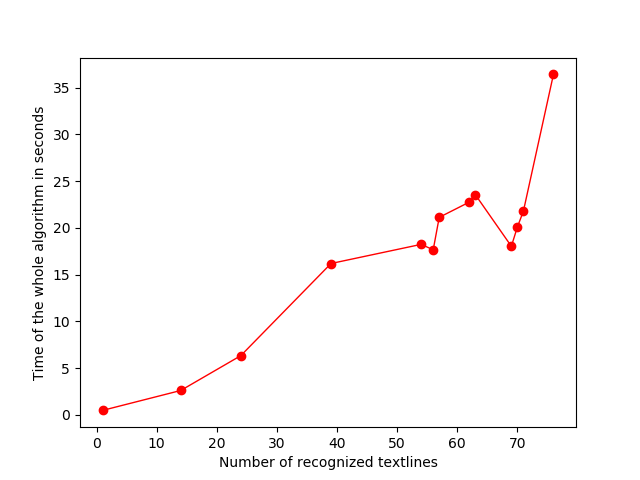
\includegraphics[width=\linewidth]{img/results/textlinesTimeAll.png}
    \caption{The overall time of execution with respect to the number of recognized textlines.}
    \label{fig:textlinesTime}
\endminipage
\label{resultsTextEffects}
\end{figure}

\section{Effects of image resolution}

The quality of the input image greatly affects Tesseract's recognition system and therefore our recognition system. Tesseract advises its users to use at least 300 dpi images, as it claims that lower resolution images are more likely to fail at recognition to a greater extent. In this section, we tested the effects of image resolution on both the speed of the algorithm (presented in~\cref{fig:dpiTessTime,fig:dpiInitTime,fig:dpiAllTime}) and the accuracy of Tesseract (by which we understand the number of recognized symbols and textlines, as Tesseract outputs barely any false positives, presented in~\cref{fig:dpiSymbols,fig:dpiTextlines}). For these purposes, we used the same different resolution images as in~\cref{resultsEffectsOfText}.

\subsection{Effects on time complexity}

From the observation of the results in~\cref{fig:dpiInitTime}, it is evident that the DPI of the image does not have a direct effect on the \texttt{init\_textlines} function. This is because the time complexity of this function is directly dependent on the number of symbols and textlines. As a higher DPI image does not necessarily mean that more symbols and textlines will be present in the image (due to false positives, incorrect splits between textlines in lower resolution images, splitting of characters and more), the dependencies presented in~\cref{fig:dpiInitTime} could greatly vary.

However, when it comes to Tesseract recognition, presented in~\cref{fig:dpiTessTime}, we can clearly see that its execution time increases with increased DPI. The exception to this is when the image has around 300 dpi, where the execution time suddenly decreases. This is due to the fact that most of the Tesseract training data are of a 300 dpi resolution (\cref{scaling}).

This implies that the overall time complexity of our algorithm will also be dependent on the DPI of the image, with the best results obtained at the DPI of around 300 (shown in~\cref{fig:dpiAllTime}). Although the recognition time is exponentially lower with the dpi under 150, the results from images with this resolution are useless, as they produce many undetected characters.

\begin{figure}[t]
\minipage{0.45\textwidth}
    \centering
    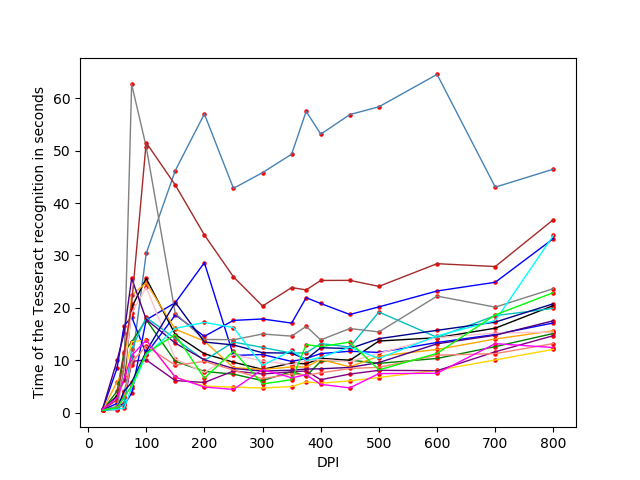
\includegraphics[width=\linewidth]{img/results/dpiTimeTesseract.png}
    \caption{The time of Tesseract recognition with respect to the DPI of the given image (different lines = different images).}
    \label{fig:dpiTessTime}
    \label{fig:textlinesTimeInit}
\endminipage\hfill
\minipage{0.45\textwidth}
    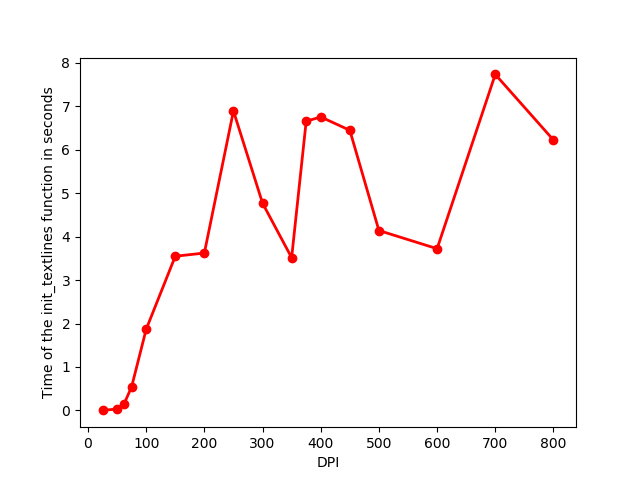
\includegraphics[width=\linewidth]{img/results/dpiTimeInit.png}
    \caption{The time of execution of the \texttt{init\_textlines} function with respect to the DPI of the given image (different lines = different images).}
    \label{fig:dpiInitTime}
\endminipage\\
\minipage{\textwidth}
    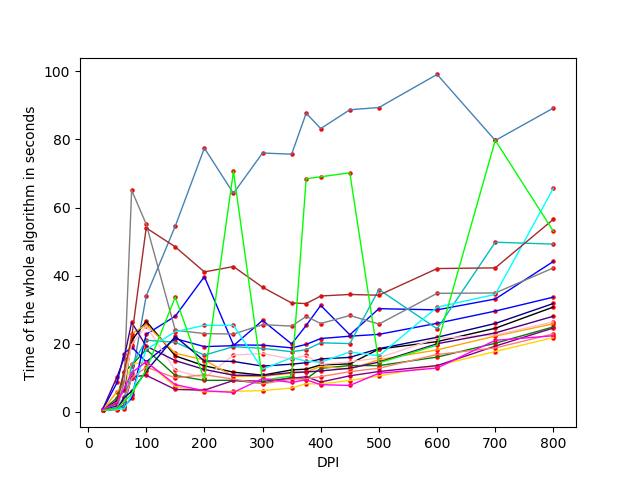
\includegraphics[width=\linewidth]{img/results/dpiTimeAll.png}
    \caption{The overall time of execution with respect to the DPI of the given image (different lines = different images).}
    \label{fig:dpiAllTime}
\endminipage
\label{resultsDPITime}
\end{figure}

\subsection{Effects on Tesseract accuracy}

From the observation of the results in~\cref{fig:dpiSymbols}, we can clearly see that the number of detected symbols rises rapidly up to the DPI of around 300. However, once we increase the DPI of the image above the value of 300, the recognition system barely recognizes any new characters. Sometimes, at significantly higher resolutions, the recognition even decreases in accuracy. This leads us to the assumption that the 300 dpi resolution is sufficient enough for symbol recognition.

As we already mentioned in this chapter, the fact that there is an increased amount of textlines does not necessarily mean that the accuracy of Tesseract has increased. Therefore, the effects of DPI on the amount of textlines in an image are unpredictable and the results presented in~\cref{fig:dpiTextlines} do not contain any meaningful information.

\begin{figure}[t]
\minipage{0.45\textwidth}
    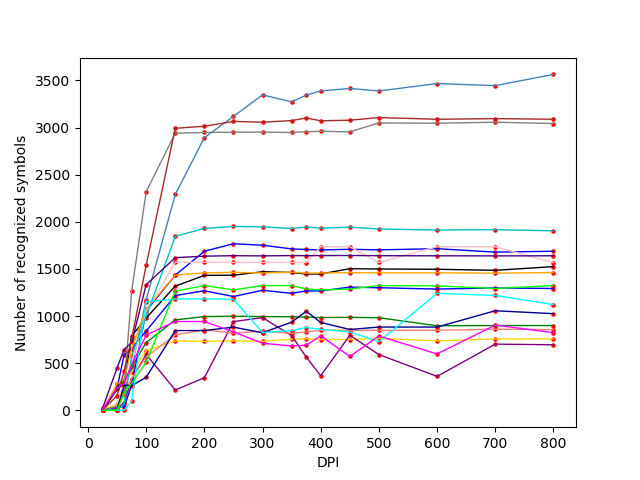
\includegraphics[width=\linewidth]{img/results/dpiSymbols.png}
    \caption{The number of recognized symbol with respect to the DPI of the given image (different lines = different images).}
    \label{fig:dpiSymbols}
\endminipage\hfill
\minipage{0.45\textwidth}
    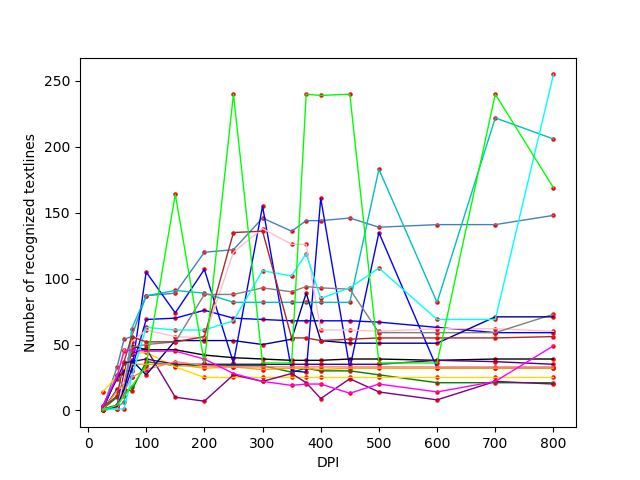
\includegraphics[width=\linewidth]{img/results/dpiTextlines.png}
    \caption{The number of recognized textlines with respect to the  DPI of the given image (different lines = different images).}
    \label{fig:dpiTextlines}
\endminipage
\label{resultsDPIAccuracy}
\end{figure}

\section{Effects of preprocessing}

As mentioned multiple times in the previous chapters, preprocessing is a crucial part of any OCR engine, including Tesseract. In both~\cref{fig:preprocessEffectsGS} and~\cref{fig:preprocessEffectsAdapt}, we present its importance along with a few examples of how the Tesseract symbol recognition results change when only slight tweaks in an image are made.

\begin{figure}[t]
\centering

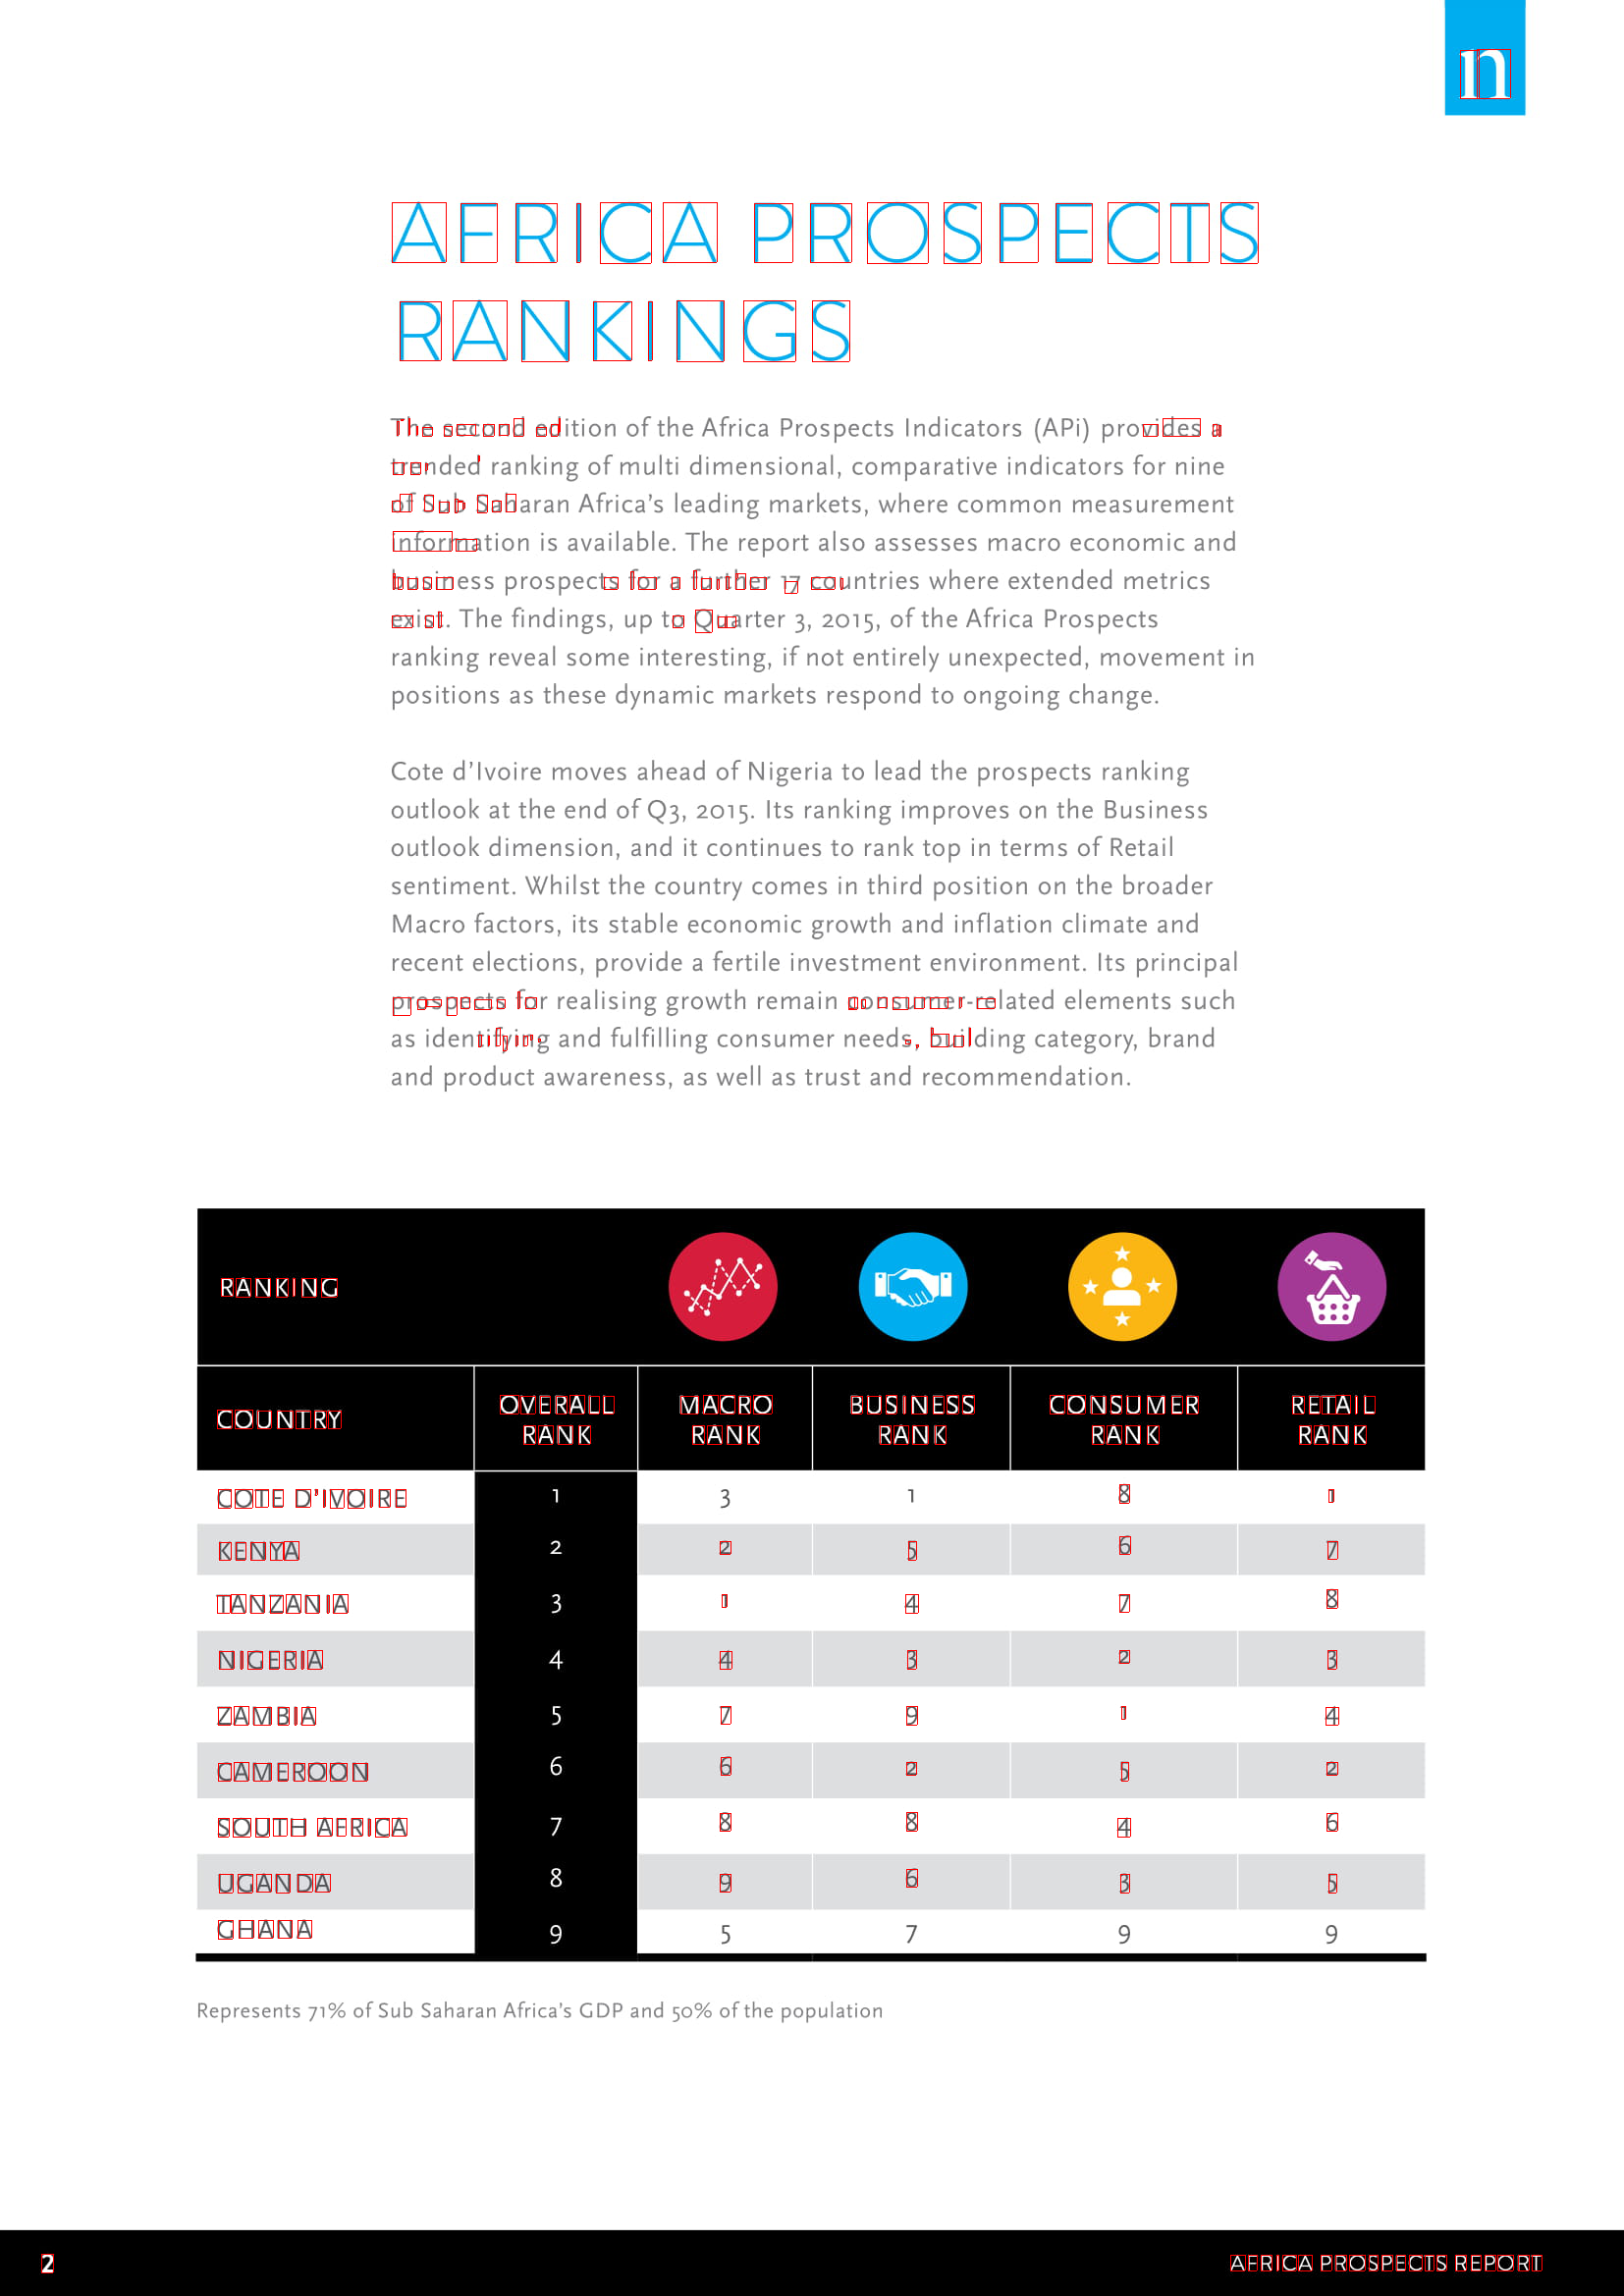
\includegraphics[width=15em]{img/results/im1_noPreproc.png}
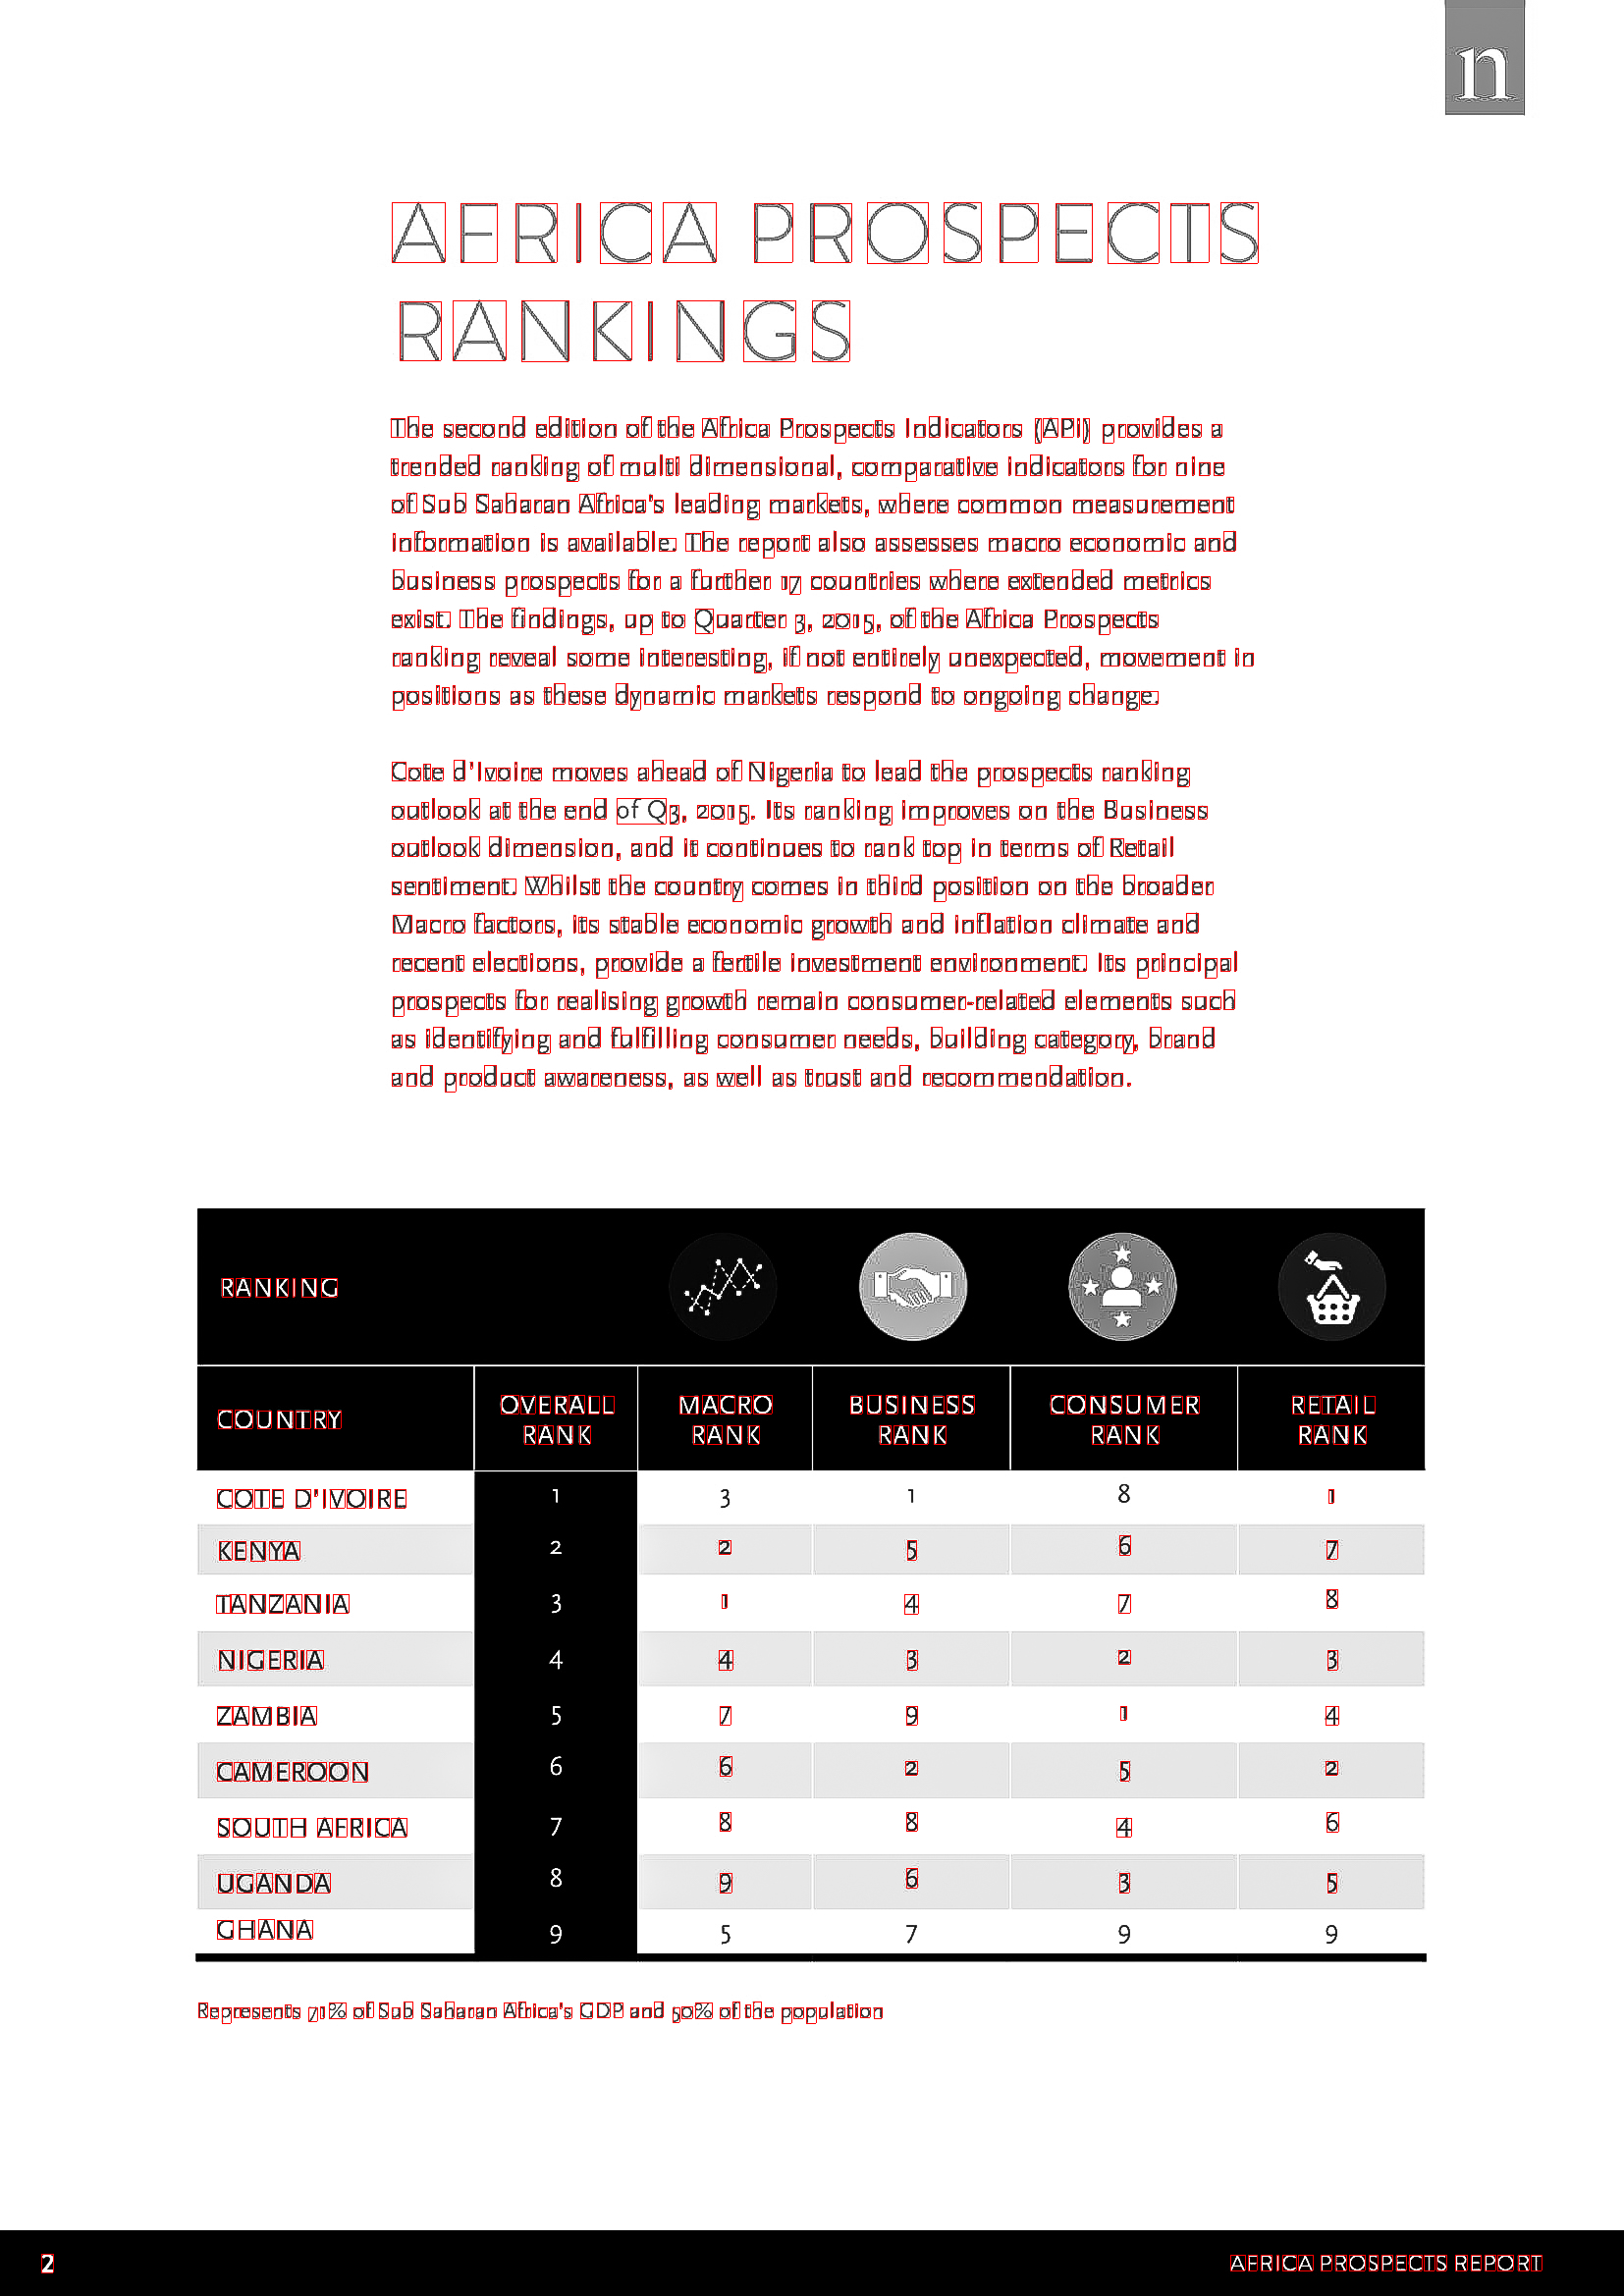
\includegraphics[width=15em]{img/results/im1_Preproc.png}

\caption{The effects of preprocessing on Tesseract recognition. Left: Tesseract does not recognize most of the symbols of the original image because of low contrast. Right: Upon applying a simple luma greyscale conversion and increasing contrast, Tesseract outputs notably better results.}
\label{fig:preprocessEffectsGS}
\end{figure}

\begin{figure}[t]
\centering

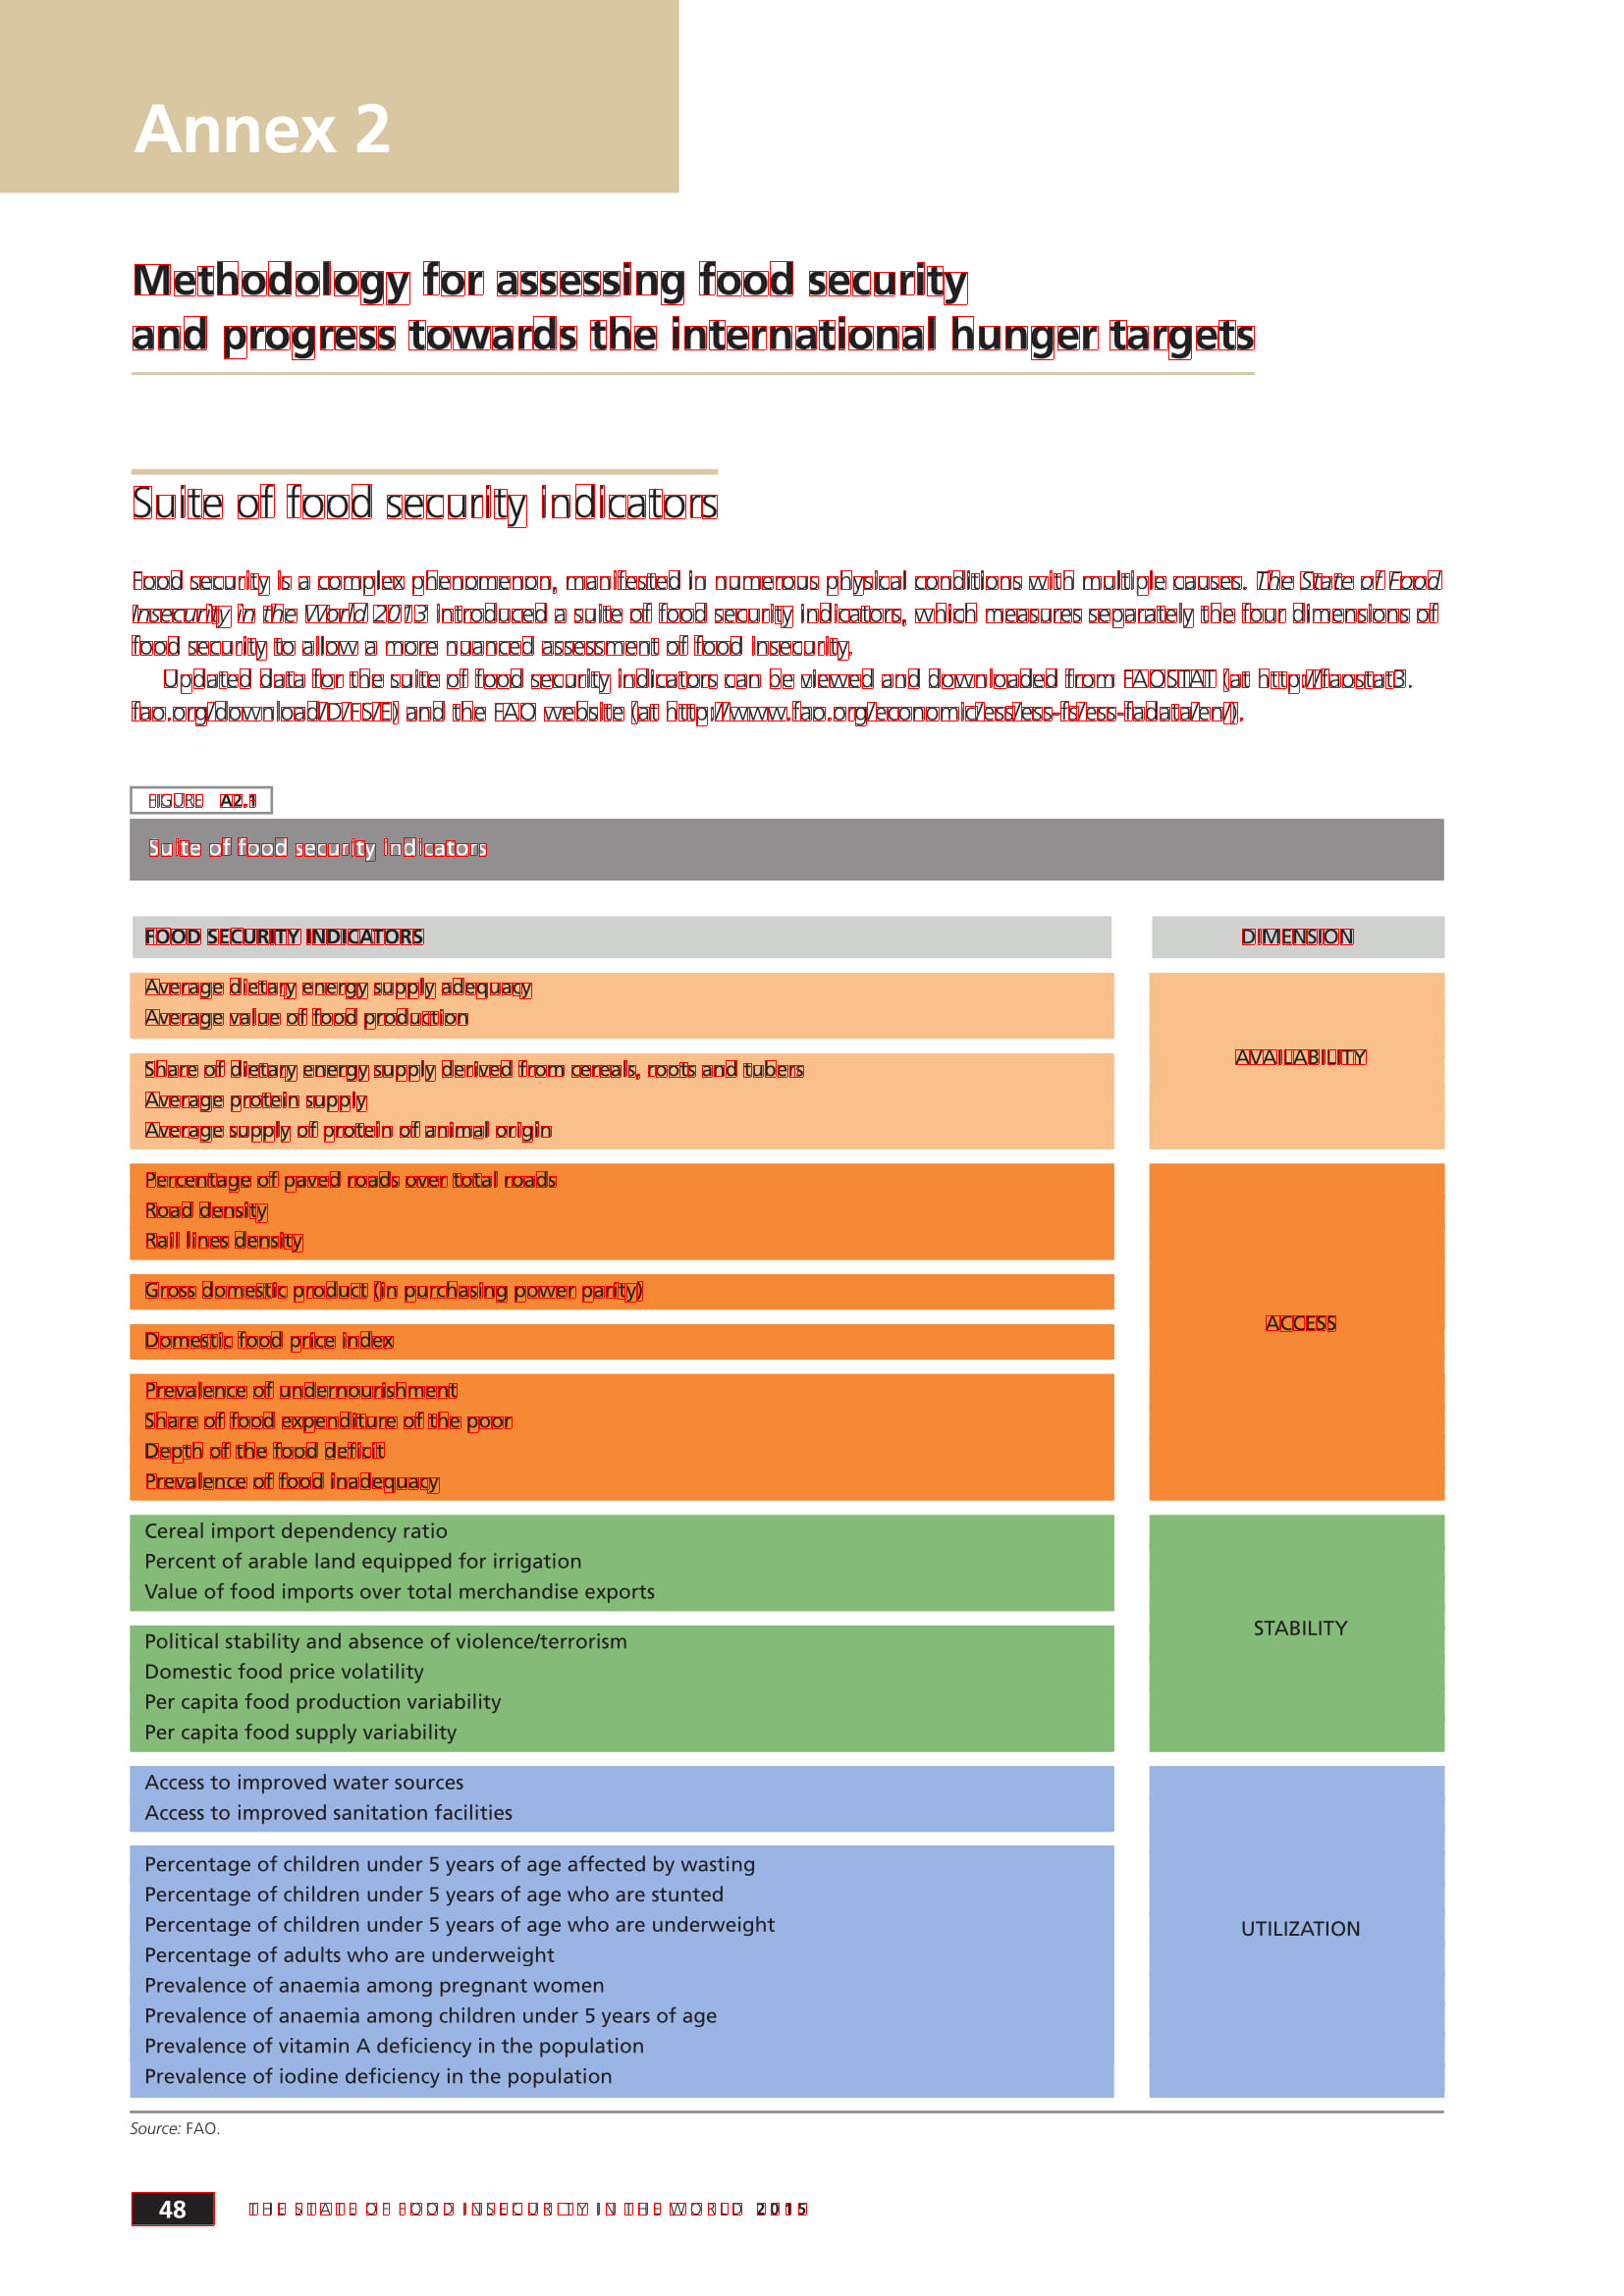
\includegraphics[width=16em]{img/results/im2_noPreproc.png}
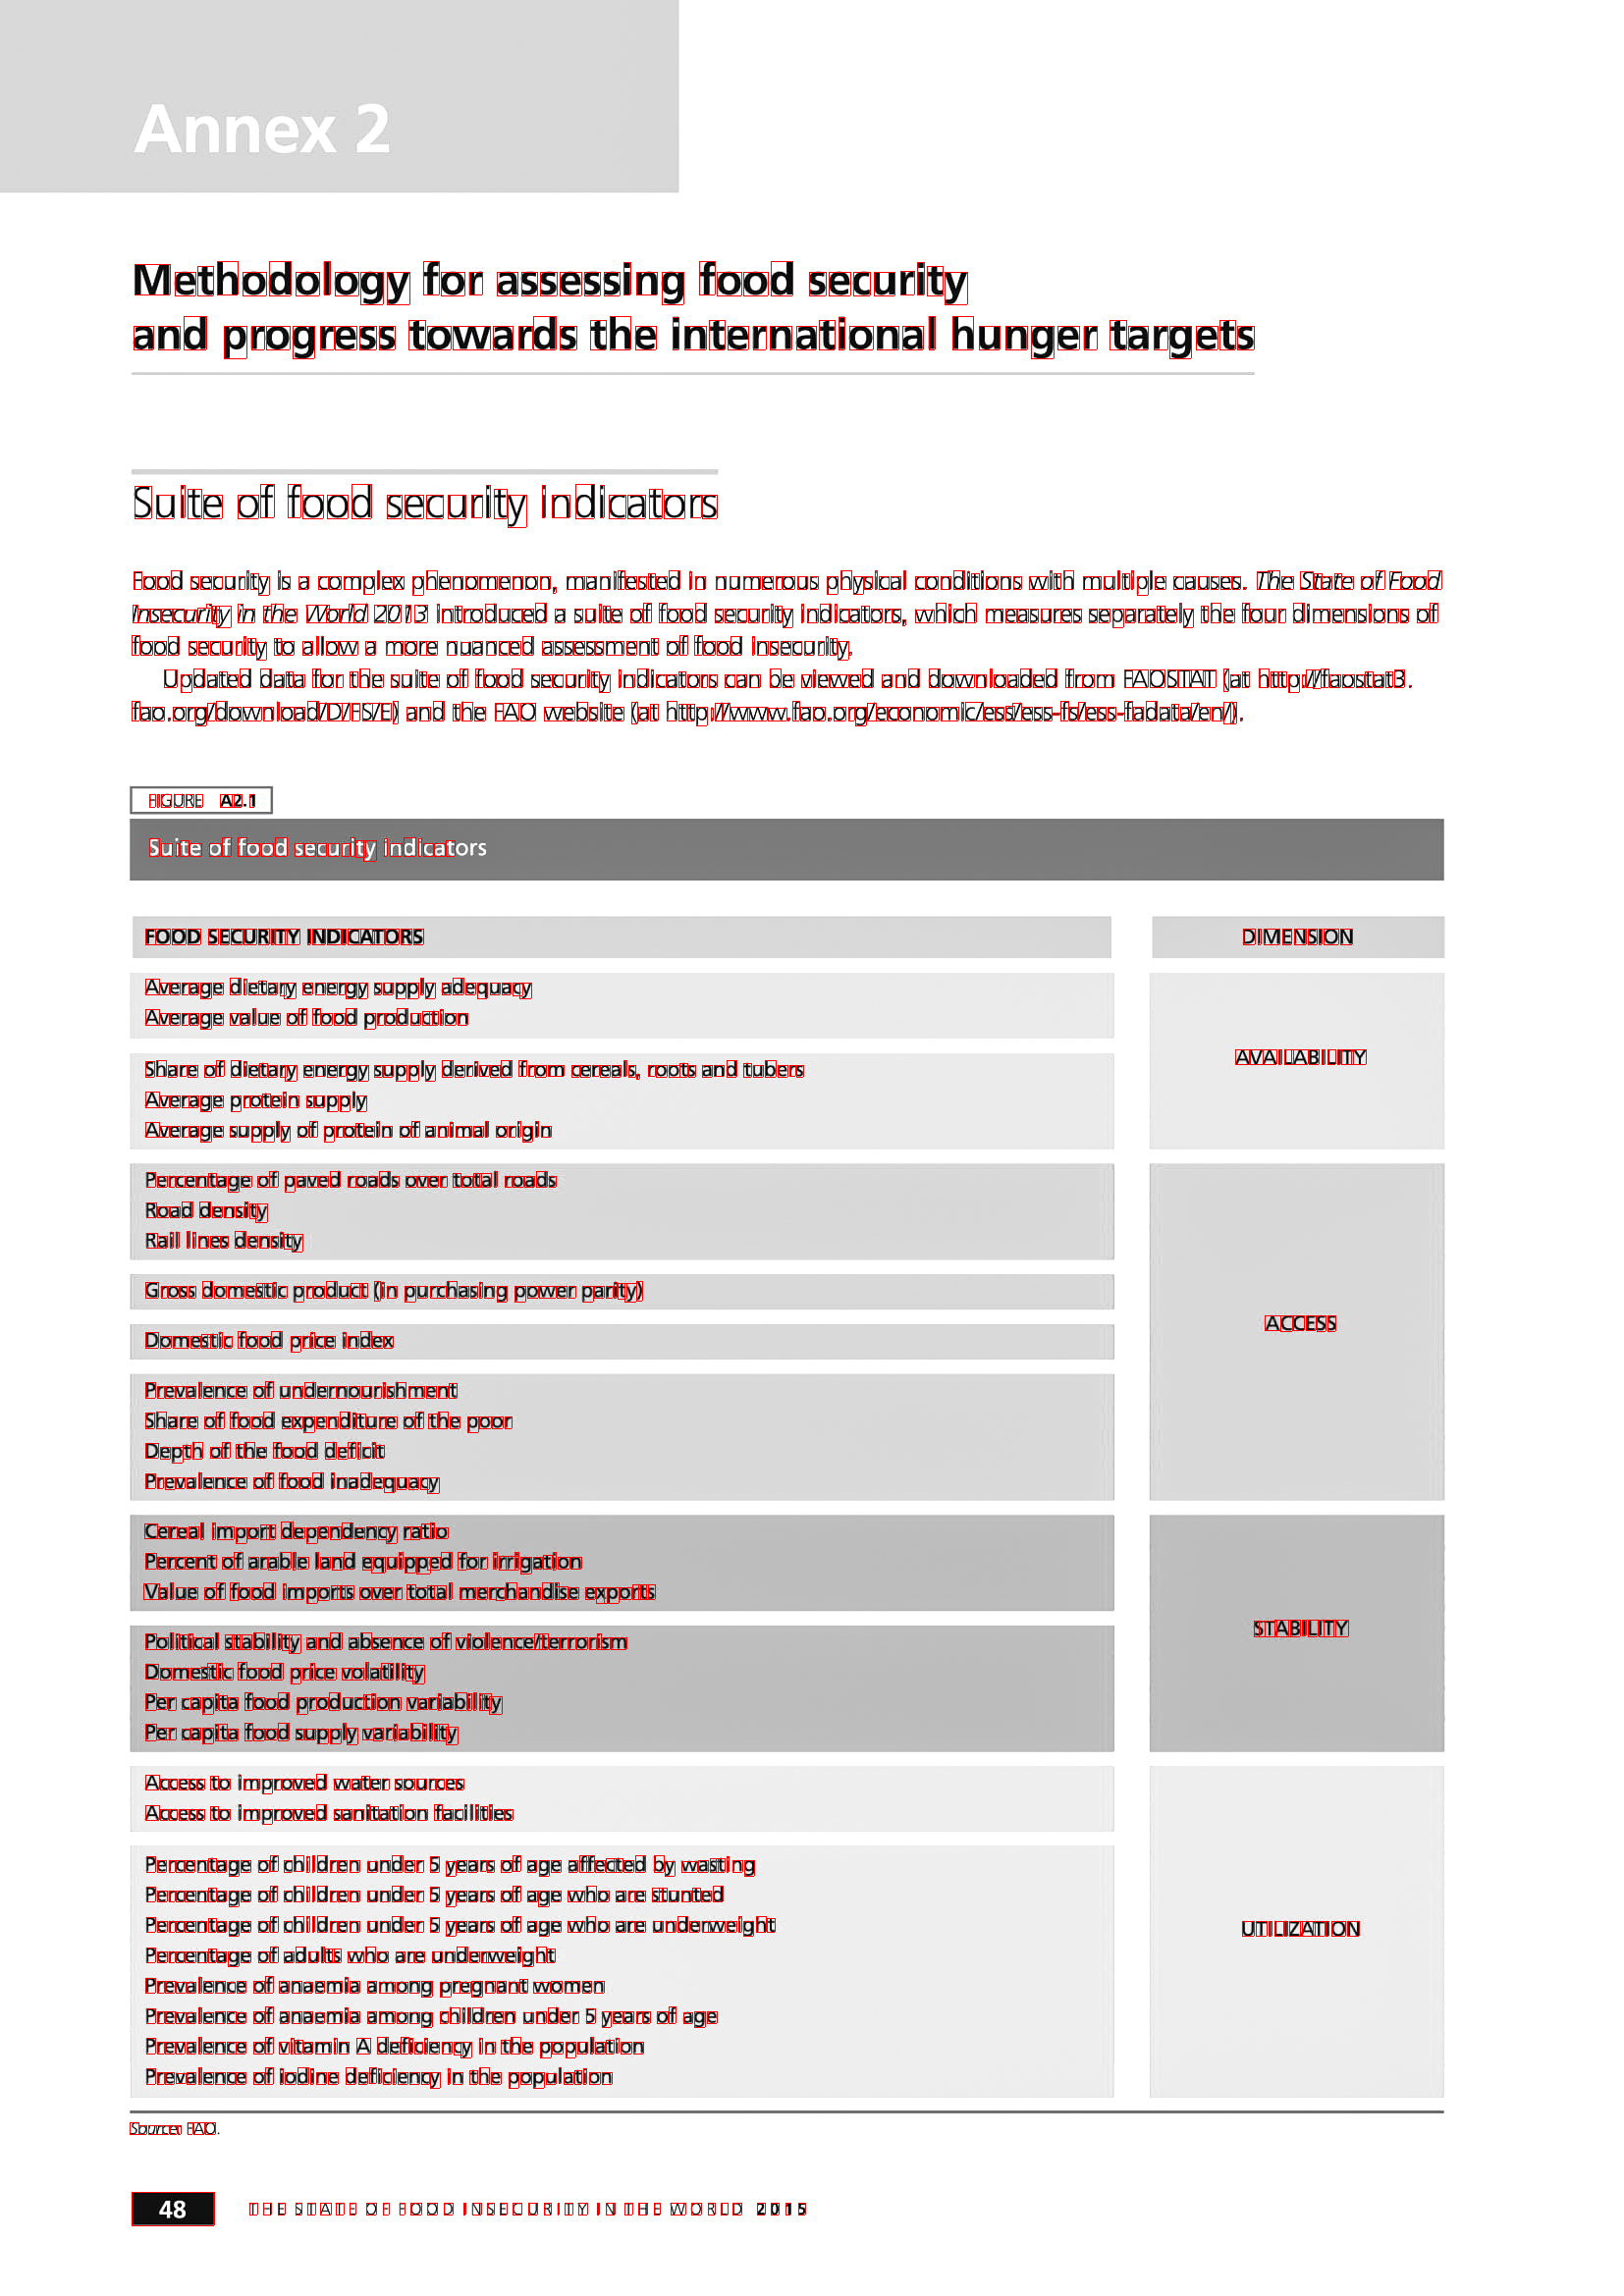
\includegraphics[width=16em]{img/results/im2_Preproc.png}

\caption{The effects of preprocessing on Tesseract recognition. Left: The lower part of the image is not recognized properly due to a dark background. Right: Tesseract recognizes all the symbols of the image once it is preprocessed by applying an adaptive greyscale conversion (by lowering blues, reds, yellows and greens).}
\label{fig:preprocessEffectsAdapt}
\end{figure}

\section{Comparison to Tesseract's TableFind} \label{resultsTableFind}

We already mentioned Tesseract's TableFind algorithm in~\cref{tableFind}. It uses heuristic algorithms to find tables from the segmentation Tesseract already offers. It also contains a simple recognition class that tries to analyze the found table for rows, columns and cells. It is a bottom-down approach, in comparison to our algorithm, which starts from the individual characters and builds up a table.

Although this algorithm has a pretty impressive results when finding tables (\emph{table detection}), it does not provide any information about the text in various cells and has no output except for a bounding box around the found table. Therefore, there is almost no support for table recognition. As this was the goal of our implementation, it is difficult to compare its results to ours. Moreover, TableFind is mainly used as a tool for developers. It has no command line interface or GUI and the user needs to understand its API to obtain its results.

The only comparable results that both algorithm produce are the recognized table. We executed both TableFind and our algorithm on all of our testing files. By observing the results, we concluded the following:
\begin{itemize}
    \item Our algorithm considers noticeably different fonts to probably not belong to the same table, which is often true. TableFind does not make this assumptions.
    \item In contrast to our algorithm, TableFind often results in over-segmentation (\cref{fig:tableFindComparison_Ours}).
    \item TableFind achieves more accurate results than our algorithm on full-page tables and heterogeneous page layouts (\cref{fig:tableFindComparison_Tess}).
    \item TableFind has no support for handling footers and often includes them in a table, in comparison to our algorithm.
    \item TableFind considers horizontal and vertical lines and therefore renders satisfactory results when it comes to bordered tables.
\end{itemize}

\begin{figure}[t]
\centering
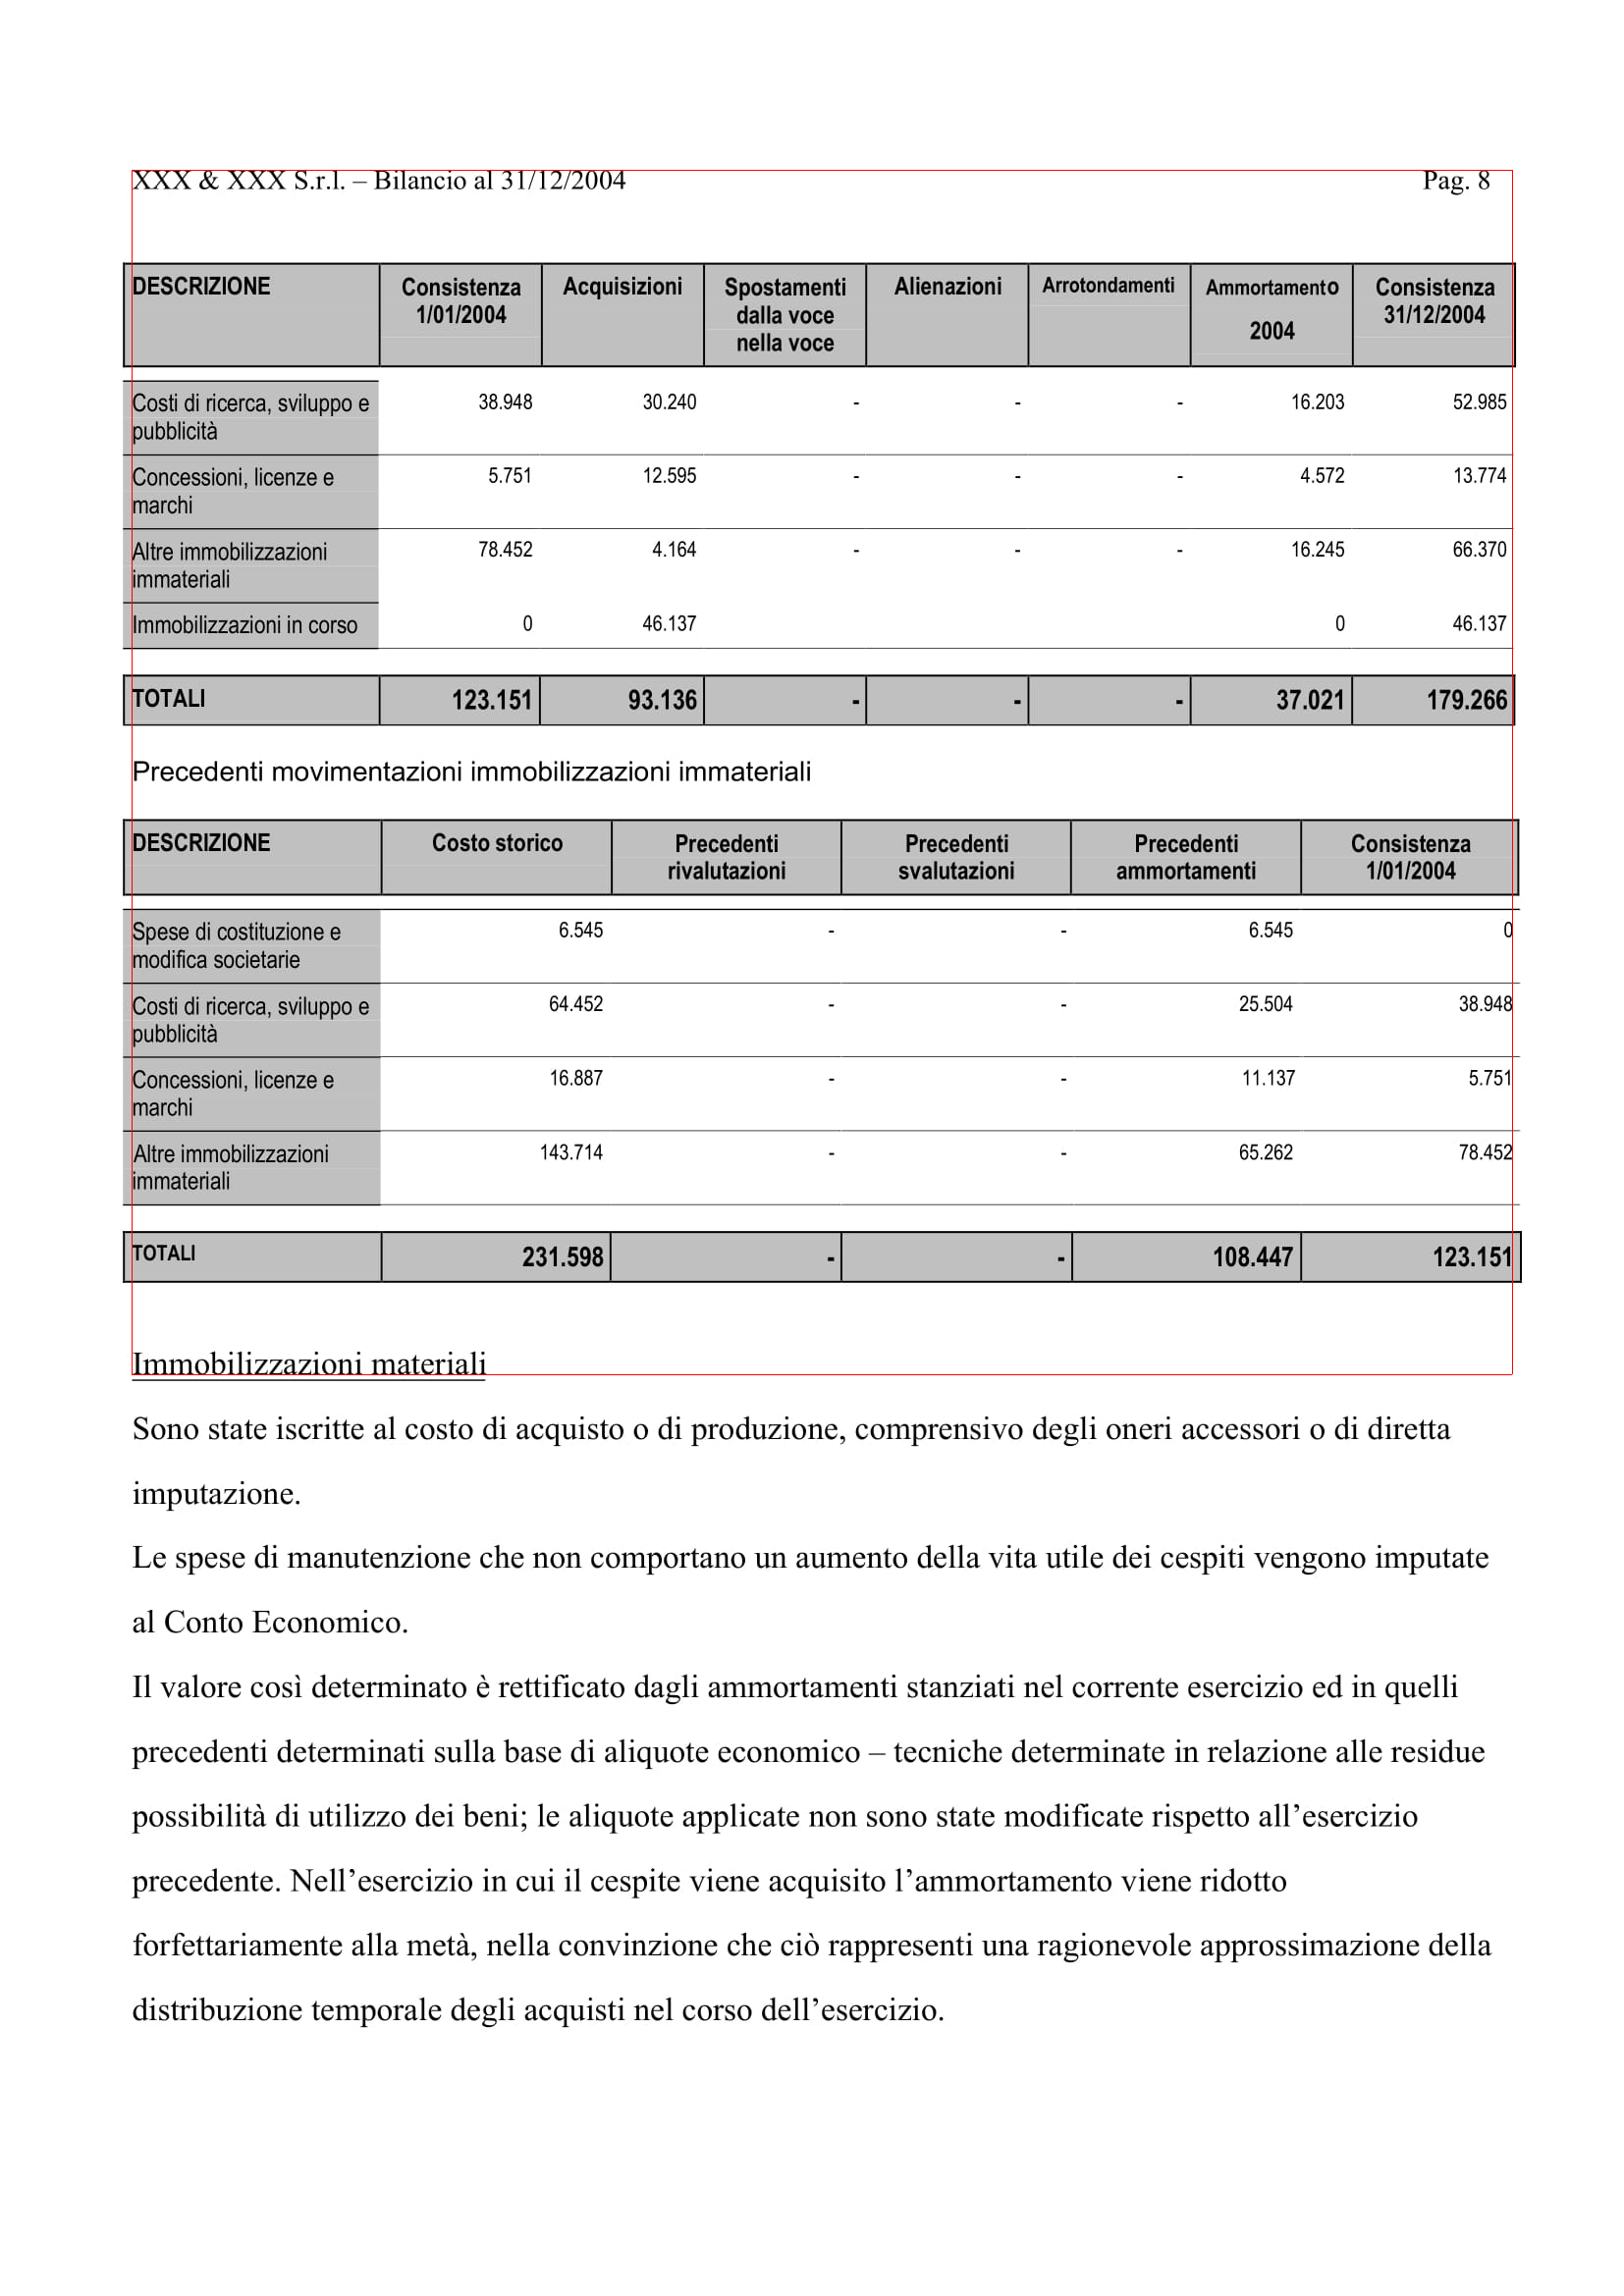
\includegraphics[width=15em]{img/results/tableFind2Tess.jpg}
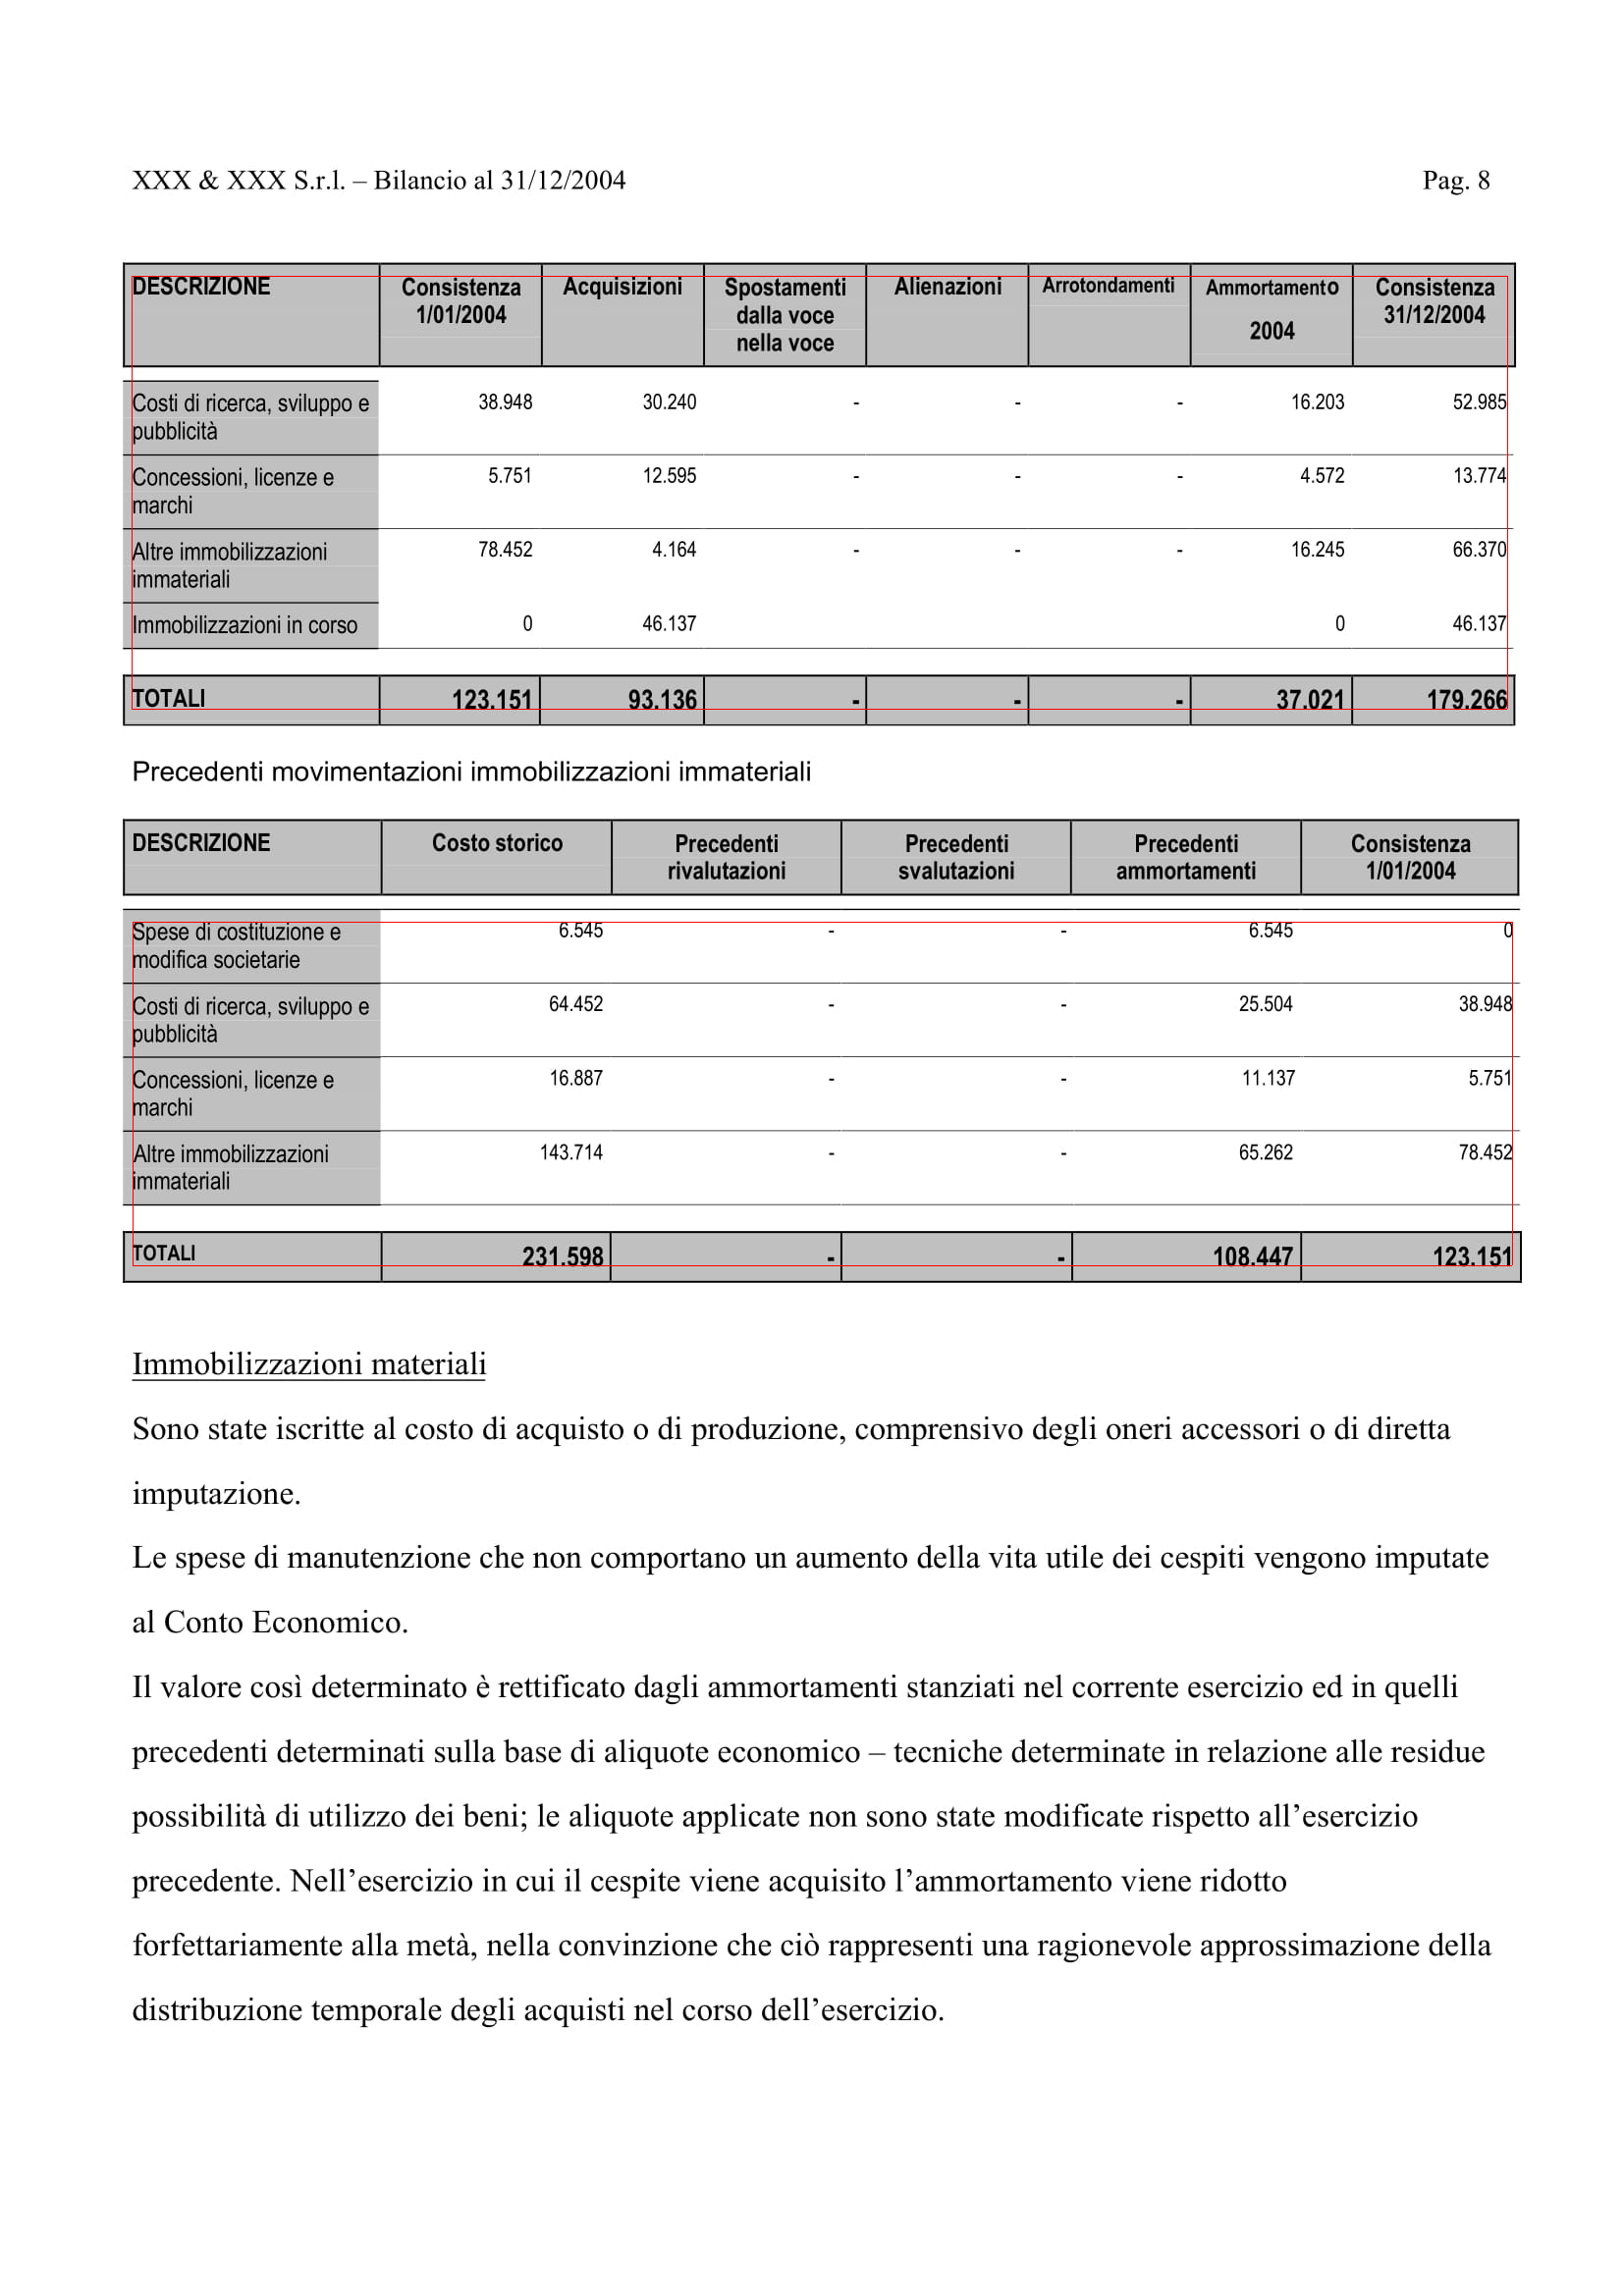
\includegraphics[width=15em]{img/results/tableFind2Us.png}
\caption{Comparison of TableFind algoritm (left) and our algoritm (right). Our algorithm renders better results in case tables are a part of a text document, while TableFind often results in over-segmentation.}
\label{fig:tableFindComparison_Ours}
\end{figure}

\begin{figure}[t]
\centering
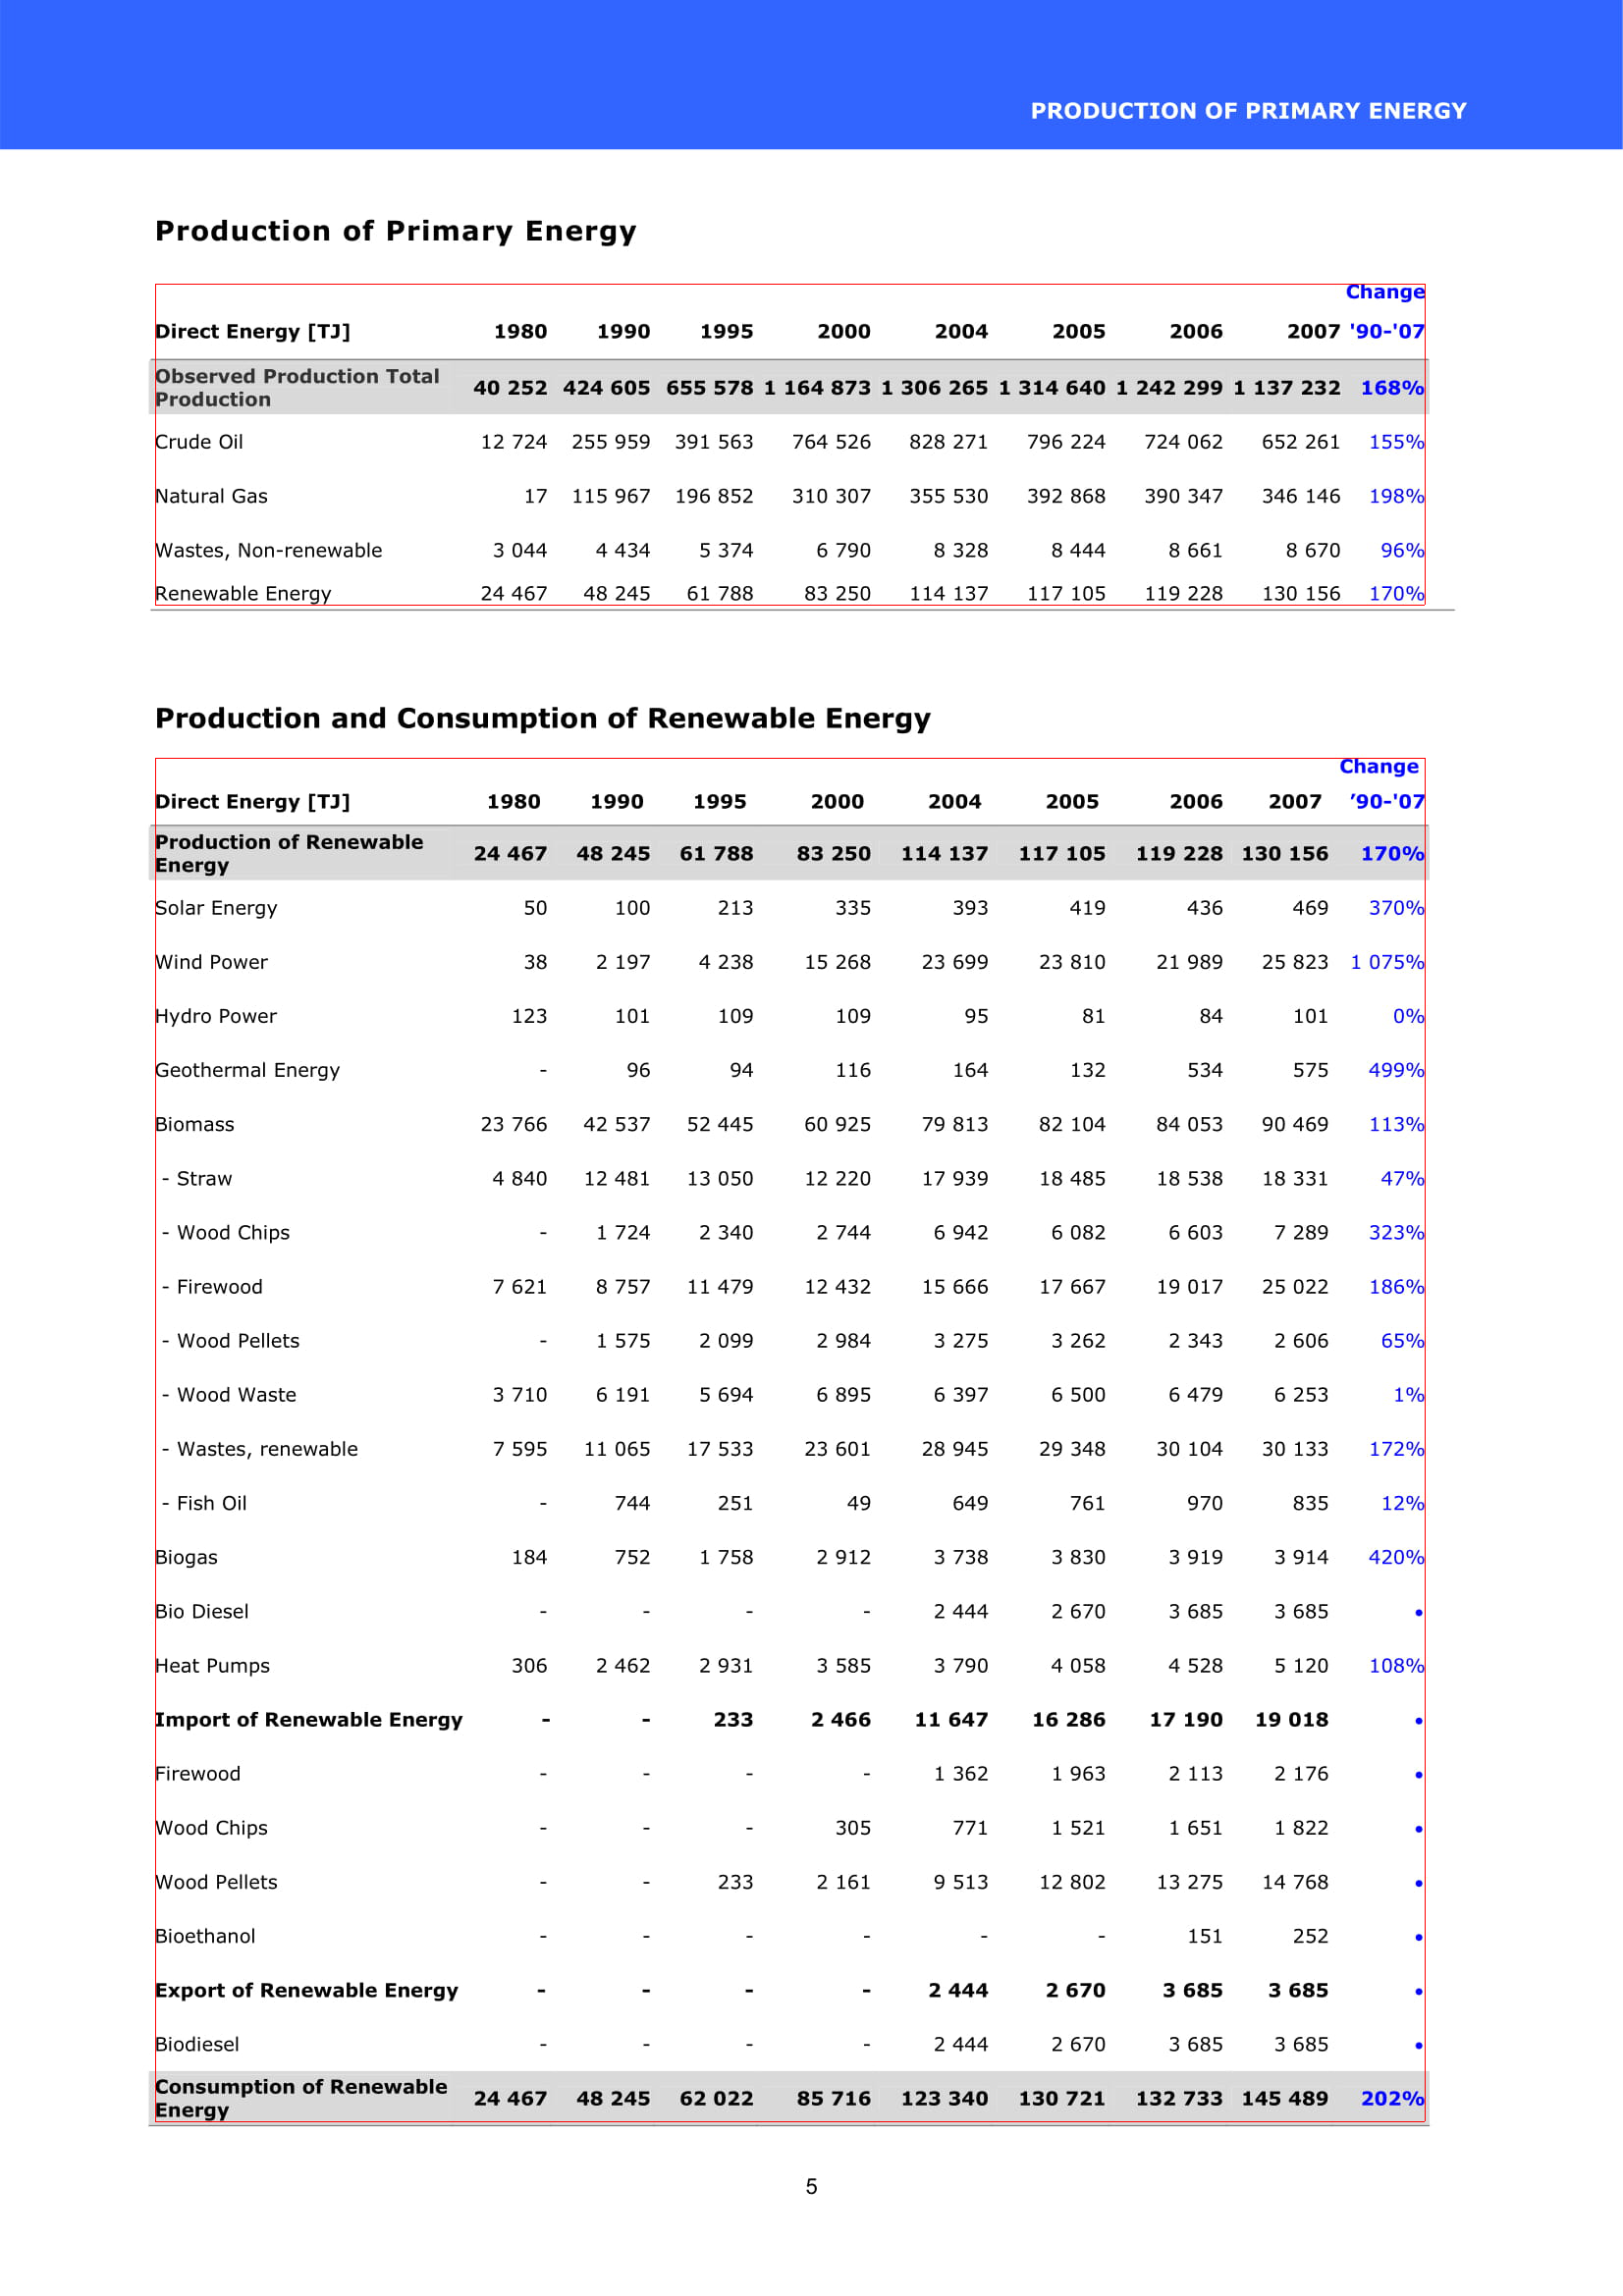
\includegraphics[width=15em]{img/results/tableFind1Tess.jpg}
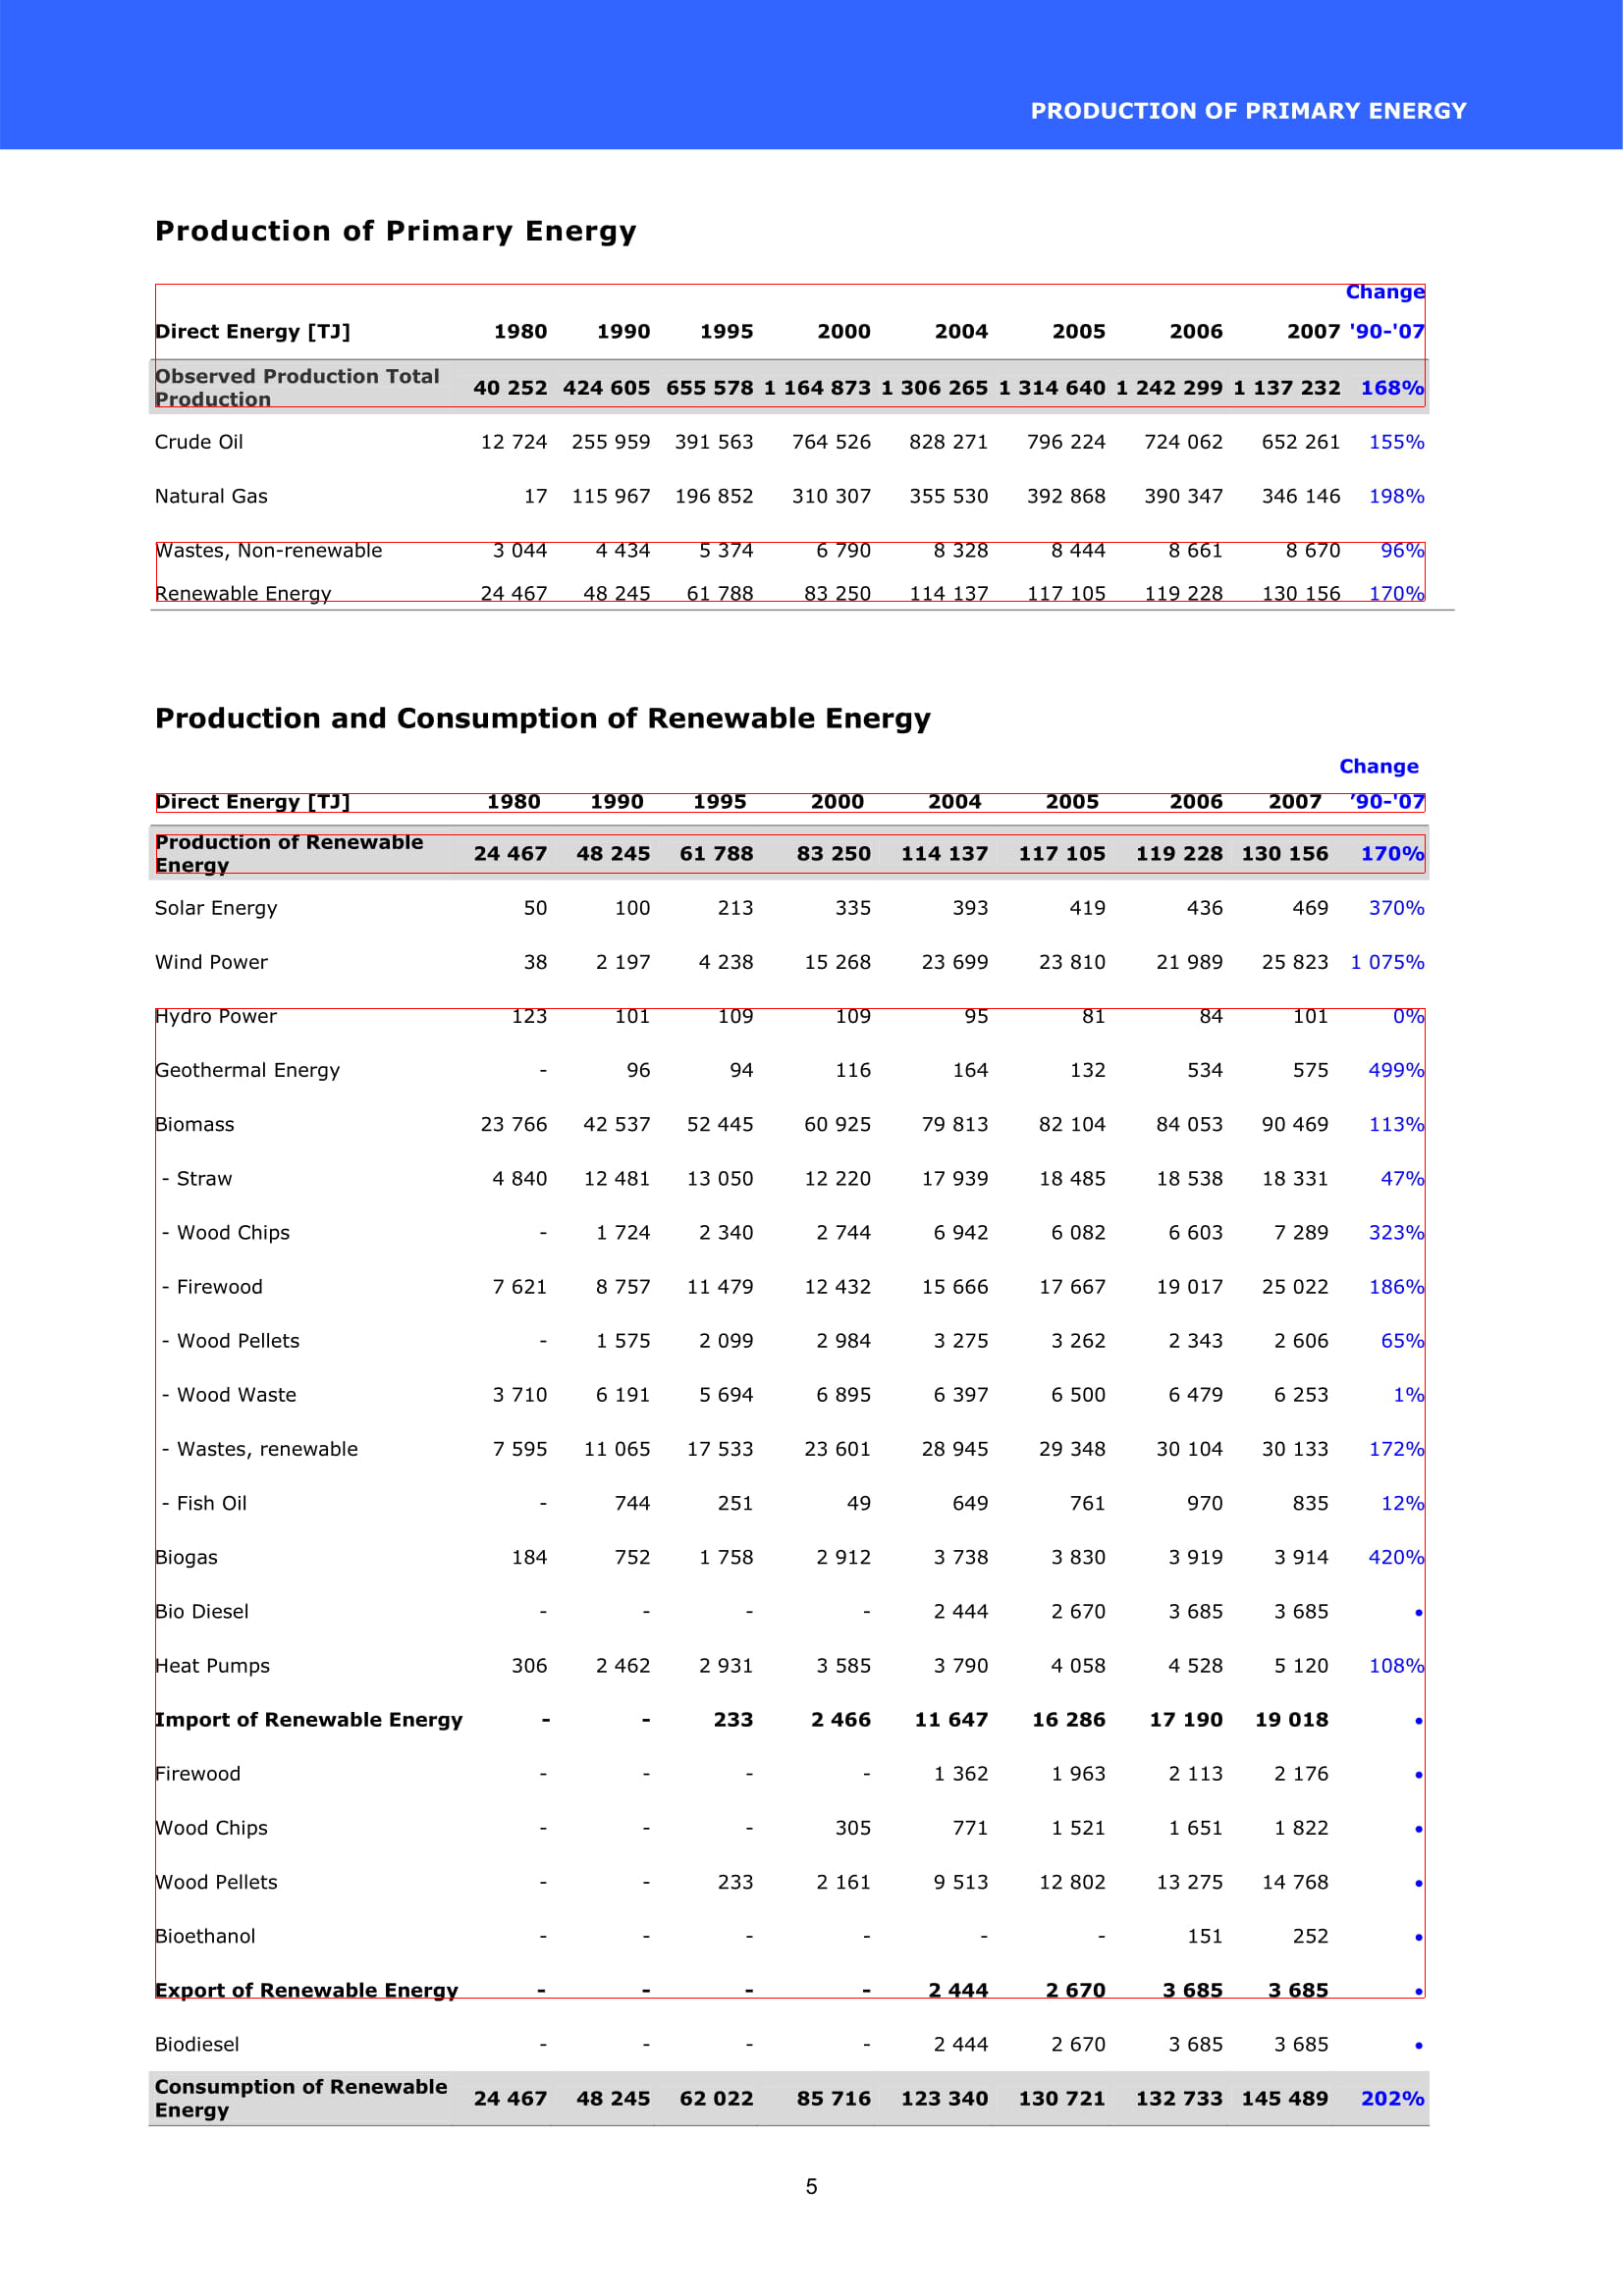
\includegraphics[width=15em]{img/results/tableFind1Us.png}
\caption{Comparison of TableFind algoritm (left) and our algoritm (right). TableFind renders notably better results when it comes to full-page tables.}
\label{fig:tableFindComparison_Tess}
\end{figure}

\section{Table recognition results}

In~\cref{fig:sampleResults}, we provide a few sample results of our algorithm. Following are the most visible problems that our algorithm encounters, along with an outline of their solutions:

\begin{itemize}
    \item \emph{Tables bordered by horizontal and vertical lines}
    
    Presented in~\cref{fig:errorTableBordered}, this most basic example of a table is something we completely ignore in our algorithm. Once we assume that a textline recognized by Tesseract is either a simple horizontal or vertical line, or even a border around a segmentation element, we automatically remove it as it may disrupt our further recognition process.
    
    Rather than ignoring these lines, we could first implement a heuristic algorithm trying to combine these lines together and determine whether they might not be representing a table.
    
    \item \emph{Word whitespace detection}

    Although column detection seems to work quite well, word whitespace detection has great room for improvement (~\cref{fig:errorWordWs}). More often than not, the estimated whitespace is greater than the real one, which results in merging of words that should be separated. As already mentioned in~\cref{columnDetection}, the approach with various font categories had better results when it came to the estimation of word whitespaces. However, we replaced this approach by the current. This was because of the complications that arose when calculating column whitespace, and because of the increased time complexity of the algorithm, as calculating the font categories involved a number of other iterations of symbols and textlines. However, to increase the accuracy of word whitespace detection, the better practice would be to use the old approach for word whitespace detection, and the new for column whitespace detection. 
    
    \item \emph{Multi-row columns}
    
    Clearly visible in~\cref{fig:errorMultiRow}, the detection of multi-rows does not work very effectively. This is because of our constant based algorithm. We could try to improve this by an implementation of a smarter algorithm based on heuristics. For example, one of the possible implementations could try to get all of the gaps between lines in a table and determine the spaces similarly to our whitespace detection (\cref{columnDetection}). Also, when every third cell's text starts with an upper case letter and all the others start with a lower case, it is a pretty clear indicator of the presence of a multi-row cell.
    
    \item \emph{Multi-column layouts}
    
    Our algorithm has no support for multi-column layouts. This results in either merging of tables from different columns into one, or recognizing each table from different column as a single column table. This can be solved by firstly checking whether the page is multi-column (by finding wide whole-page columns that contain no symbols), and then applying our algorithm to each of the recognized columns.
    
    \item \emph{Different languages support}
    
    In our implementation, we initialize Tesseract with a testing data set suitable for characters of English language. Tesseract still recognizes symbols from other languages (like é, ô, ñ and many more), but instead of outputting the symbol we wished for, it returns a combination of non-alphabetical ASCII characters. Although this does not interfere with the image output of our table recognition, it notably affects the json output.
    
    This can be solved by adding other testing data from the Tesseract open source repository and implementing their usage.
    
    \item \emph{Support of only simple table structure}
    
    Our system does not recognize complicated table structures (\cref{fig:errorTableStructures}). It relies on tables having a simple grid layout. Moreover, the structure of our algorithm was not designed for handling other kinds of layouts  (although our JSON output file supports them). Therefore, to solve this problem, a lot of serious changes need to be made in our function that merges lines into tables, such as isolating the tables, checking for their headers, adding the support for segmentation of the table and maybe even a semantic analysis.
    
    \item \emph{Other errors}
    
    Our algorithm encounters multiple other types of errors. These include unrecognized headers of tables, table splits, recognition of graphics as tables, no support for vertical text and others. We present a few of them in~\cref{fig:errorsOtherSplit,fig:errorsOtherGraphics,fig:errorsOtherHeaders}.
    
\end{itemize}

\begin{figure}[t]
\centering
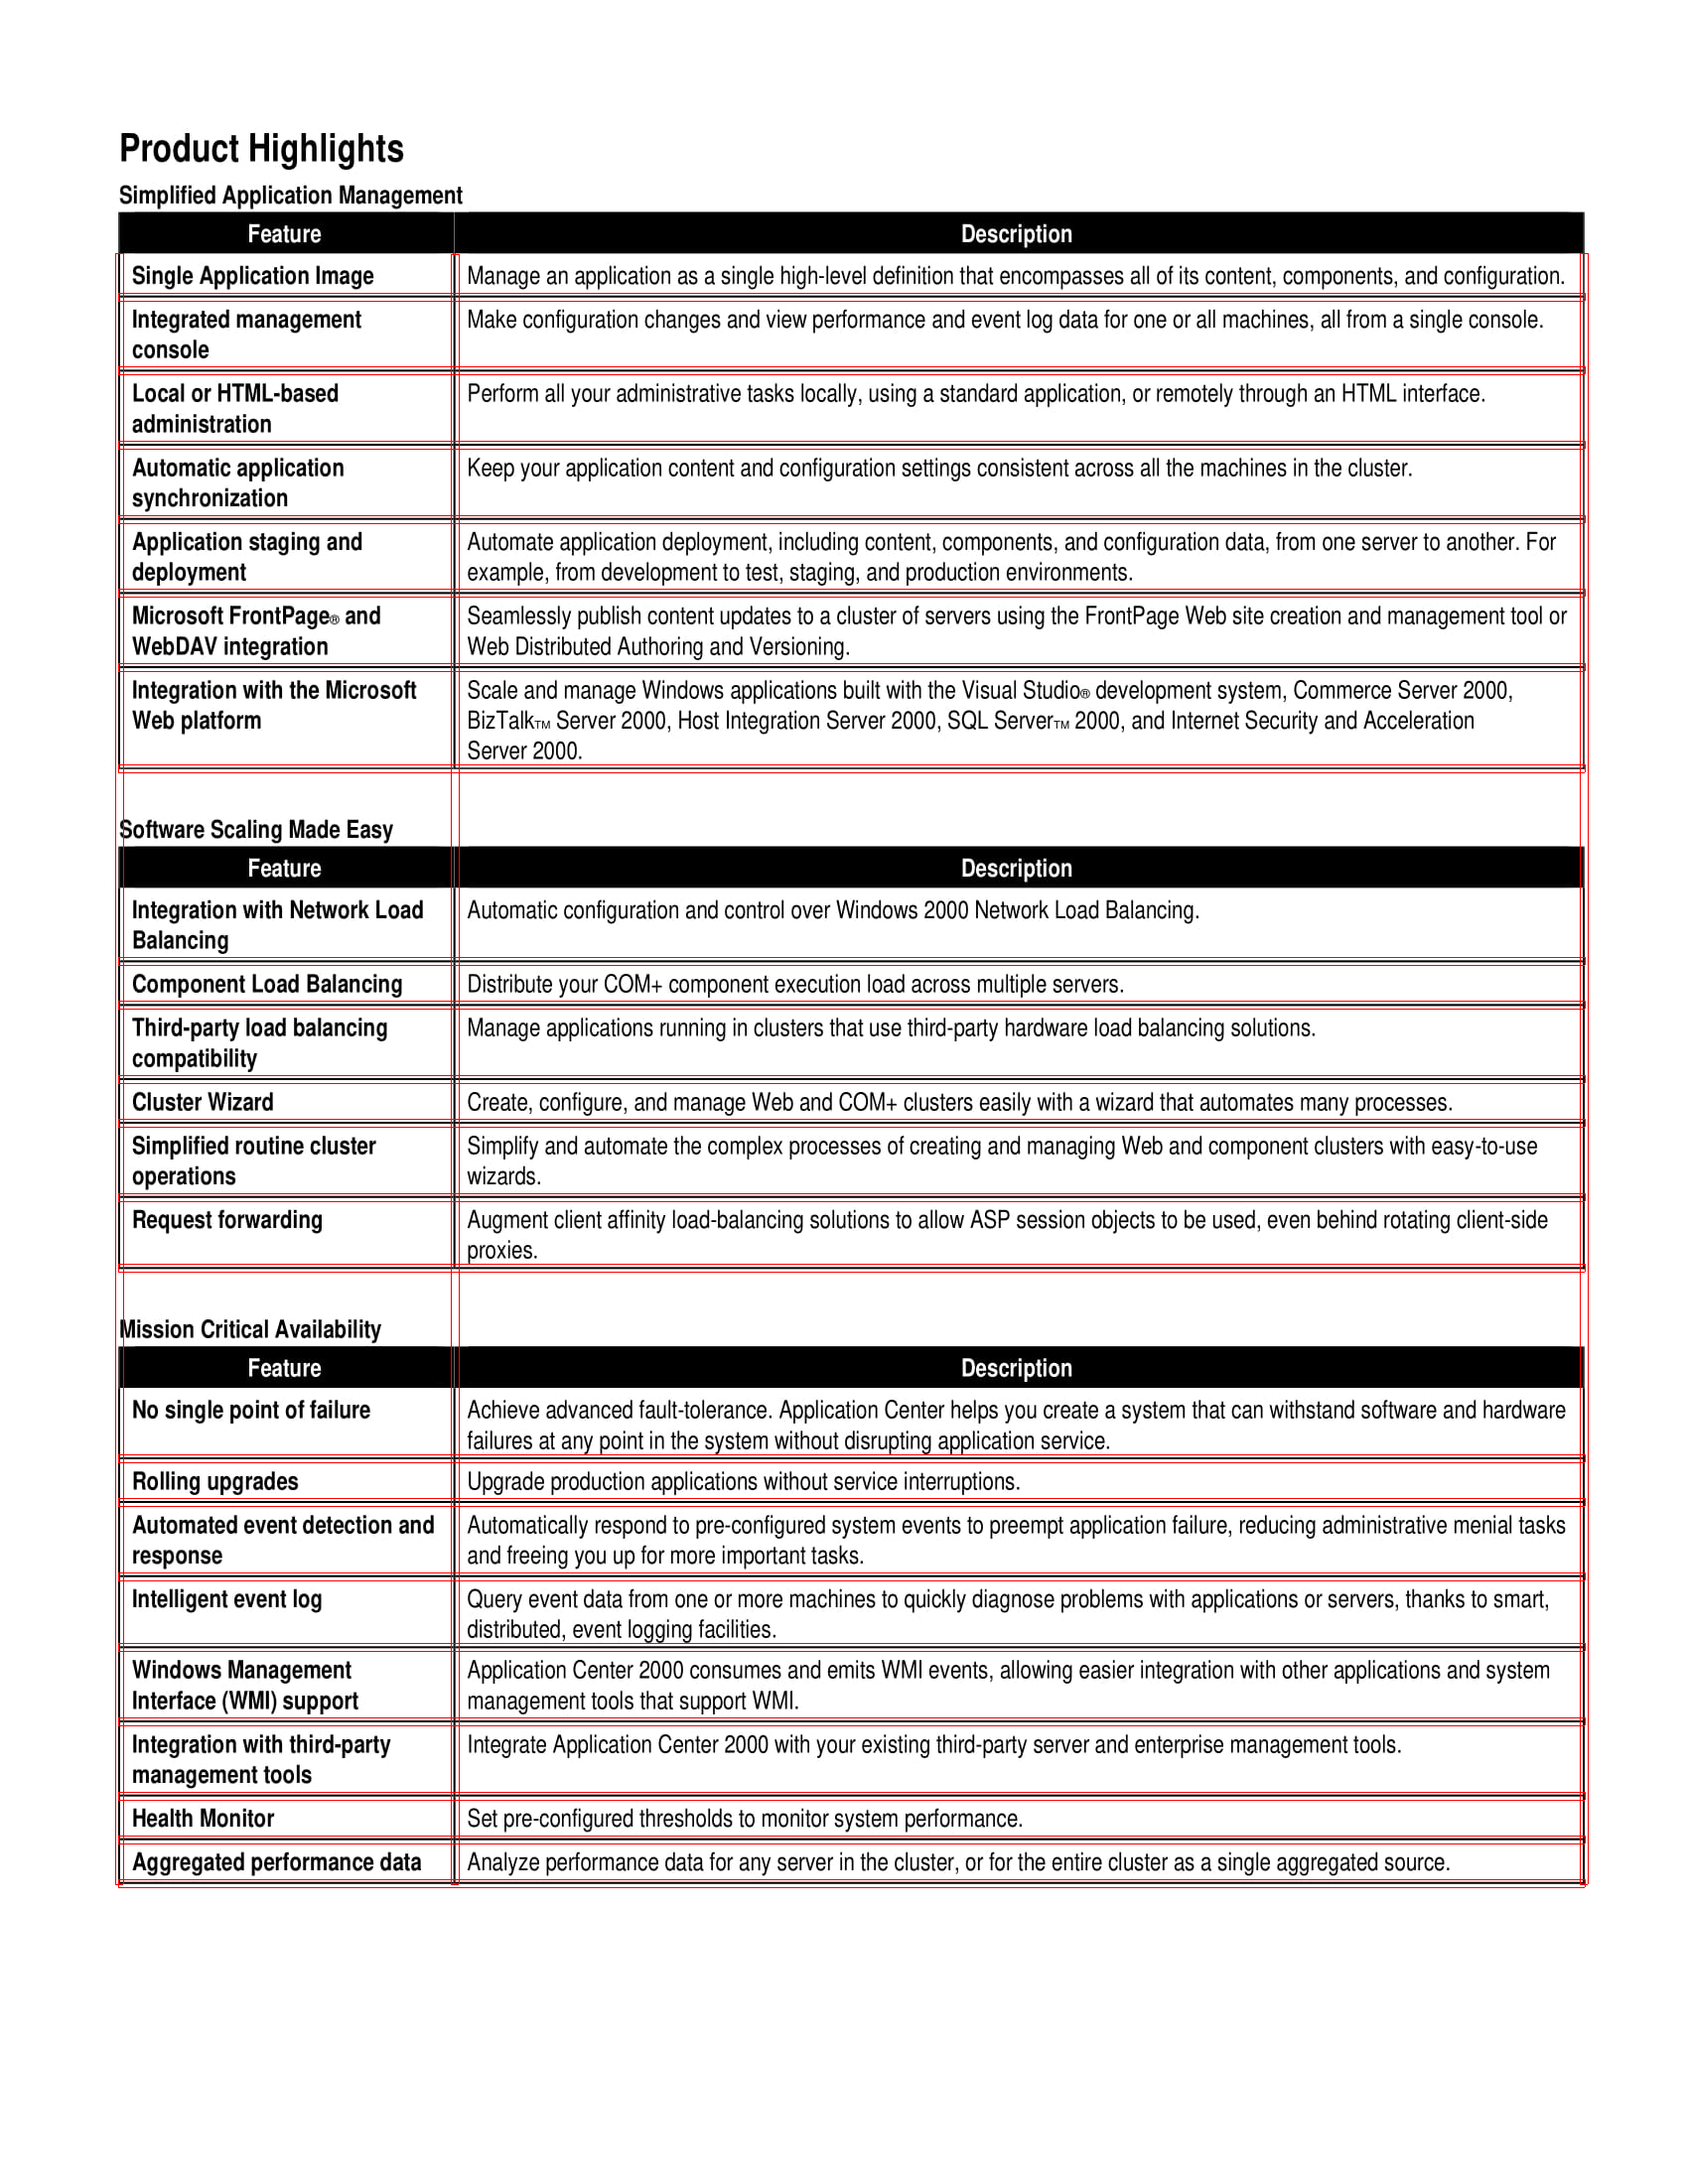
\includegraphics[width=20em]{img/results/errorTableBordered.png}
\caption{Empty horizontal and vertical lines recognized by the Tesseract textline recognition. In our algorithm, we remove them and in the end, our algorithm determines there is no table present in the image. With the use of these lines, table recognition could significantly improve.}
\label{fig:errorTableBordered}
\end{figure}

\begin{figure}[t]
\centering
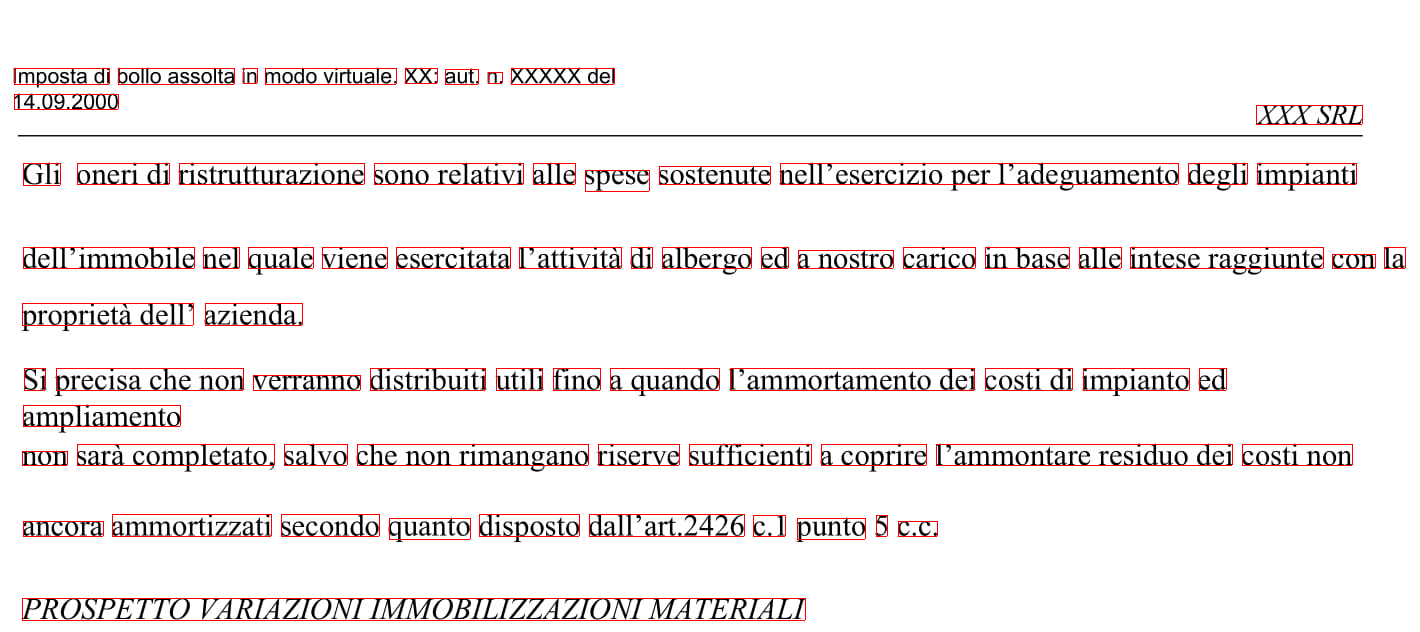
\includegraphics[width=20em]{img/results/errorWordWhitespace.png}
\caption{Improperly recognized words in a text. The biggest issue is that multiple words are often merged into one.}
\label{fig:errorWordWs}
\end{figure}

\begin{figure}[t]
\centering
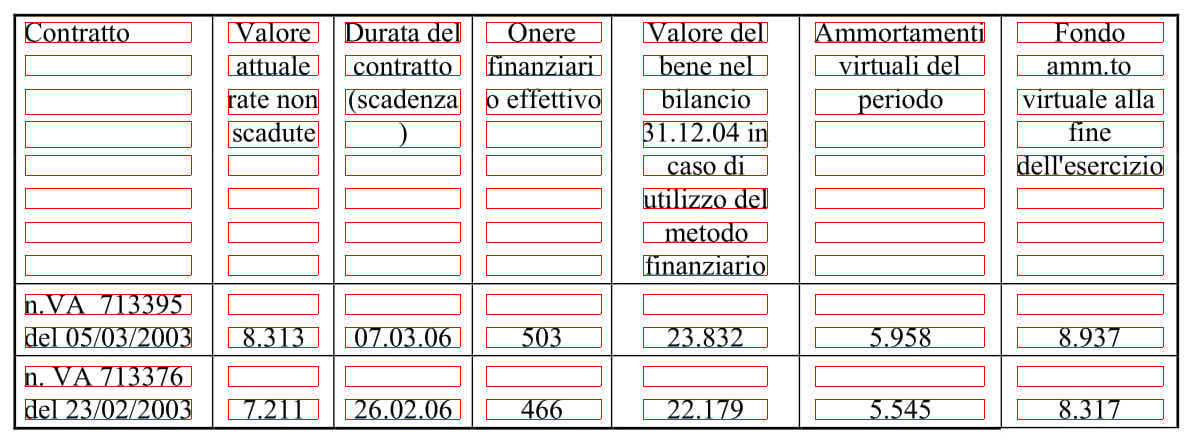
\includegraphics[width=20em]{img/results/errorMultiRow.png}
\caption{Improperly recognized multi-row cells.}
\label{fig:errorMultiRow}
\end{figure}

\begin{figure}[t]
\centering
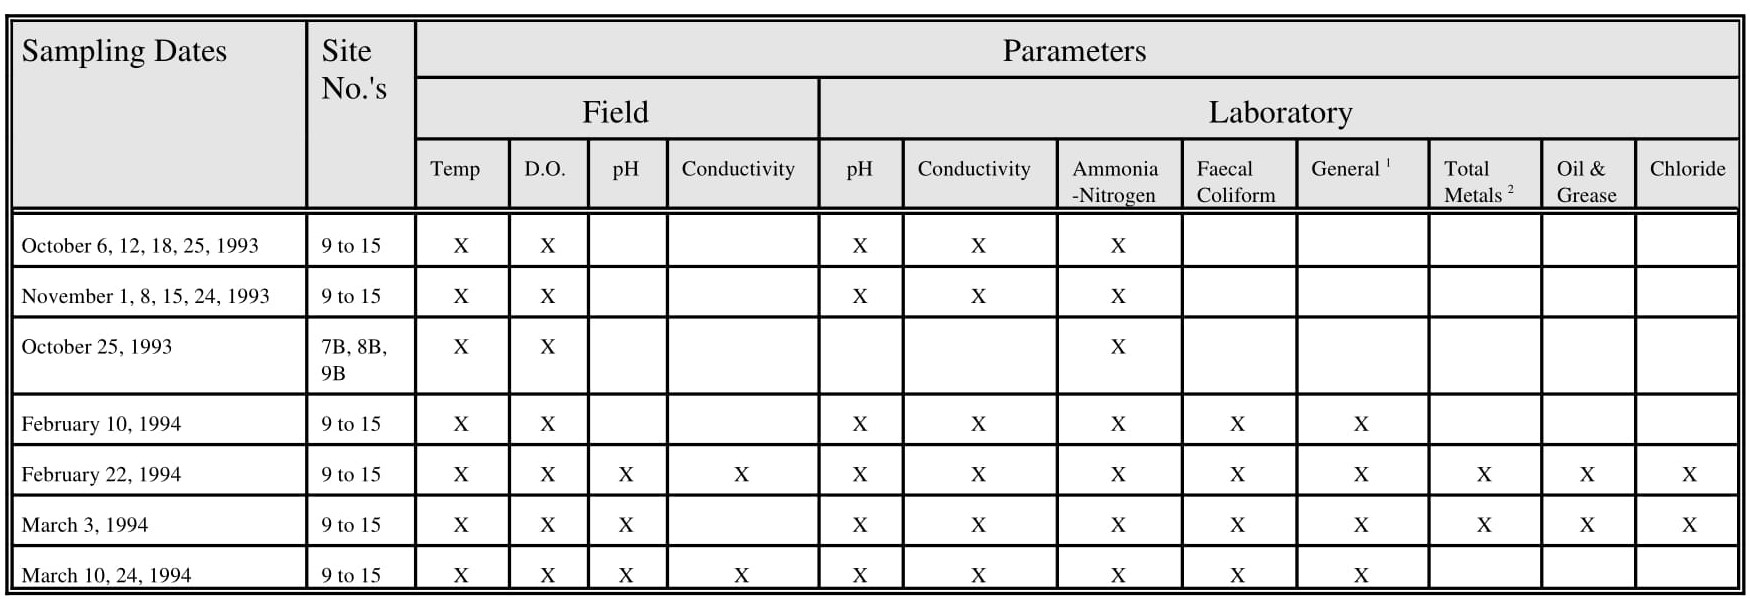
\includegraphics[width=20em]{img/results/errorStructure.jpg}
\caption{Complicated table structure.}
\label{fig:errorTableStructures}
\end{figure}

\begin{figure}[t]
\centering

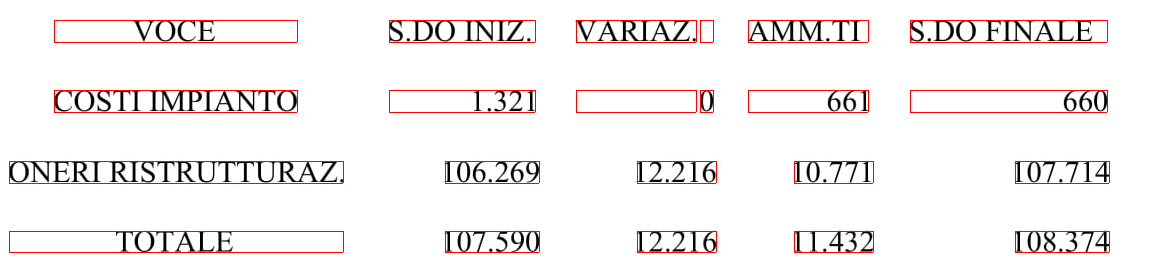
\includegraphics[width=15em]{img/results/otherErr1Cell.png}
\qquad
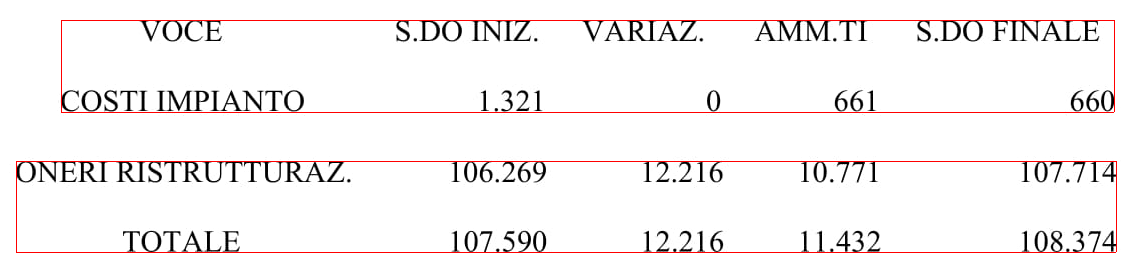
\includegraphics[width=15em]{img/results/otherErr1Table.png}

\caption{Table split errors. Although the image contains only one table, two are recognized. Our algorithm assumes that the first table has 6 columns, while the second has only 5 which do not align properly.
Left: recognized tables by cells; right: borders of the recognized tables.}
\label{fig:errorsOtherSplit}
\end{figure}

\begin{figure}[t]
\centering
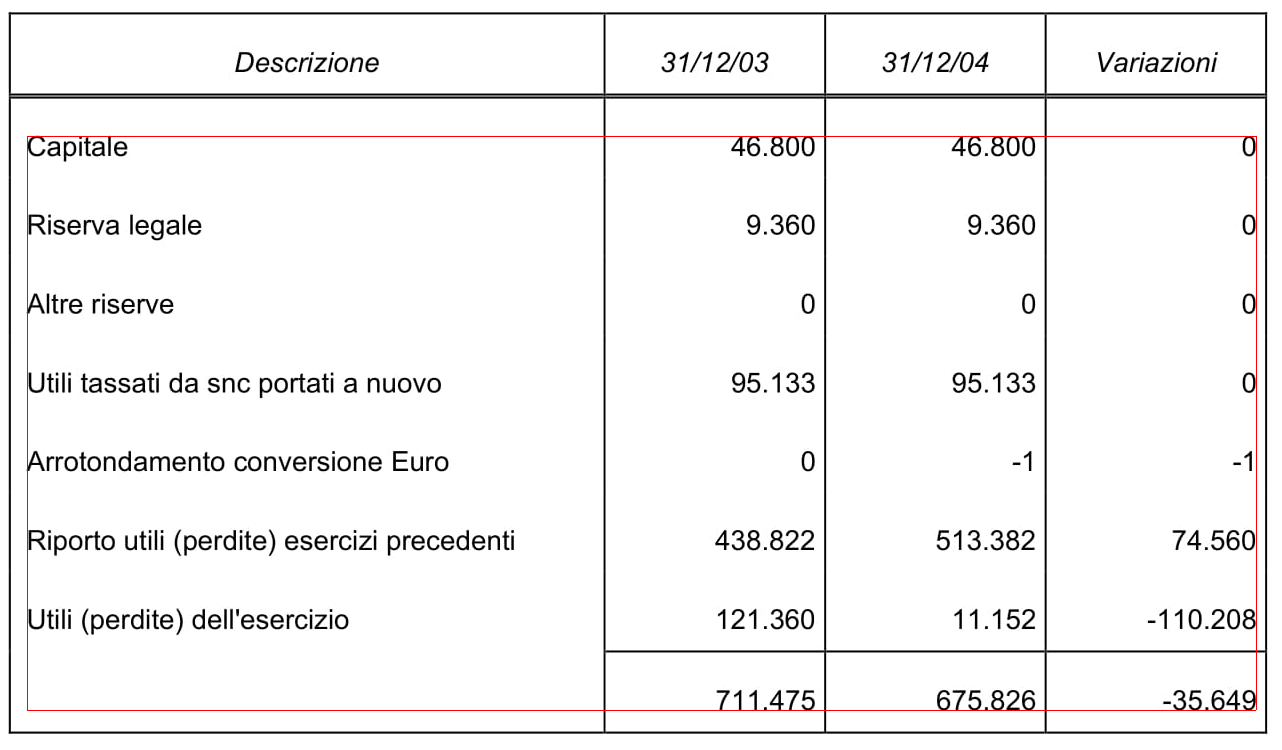
\includegraphics[width=15em]{img/results/otherErr2.png}
\caption{Unrecognized table headers.}
\label{fig:errorsOtherHeaders}
\end{figure}

\begin{figure}[t]
\centering
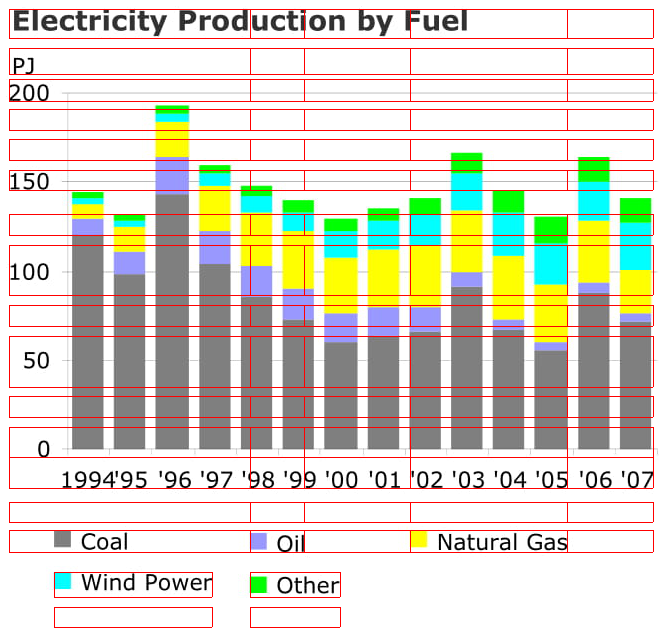
\includegraphics[width=15em]{img/results/otherErr3.png}
\caption{Our algorithm's influence on graphics images.}
\label{fig:errorsOtherGraphics}
\end{figure}

\begin{figure}[t]
\centering
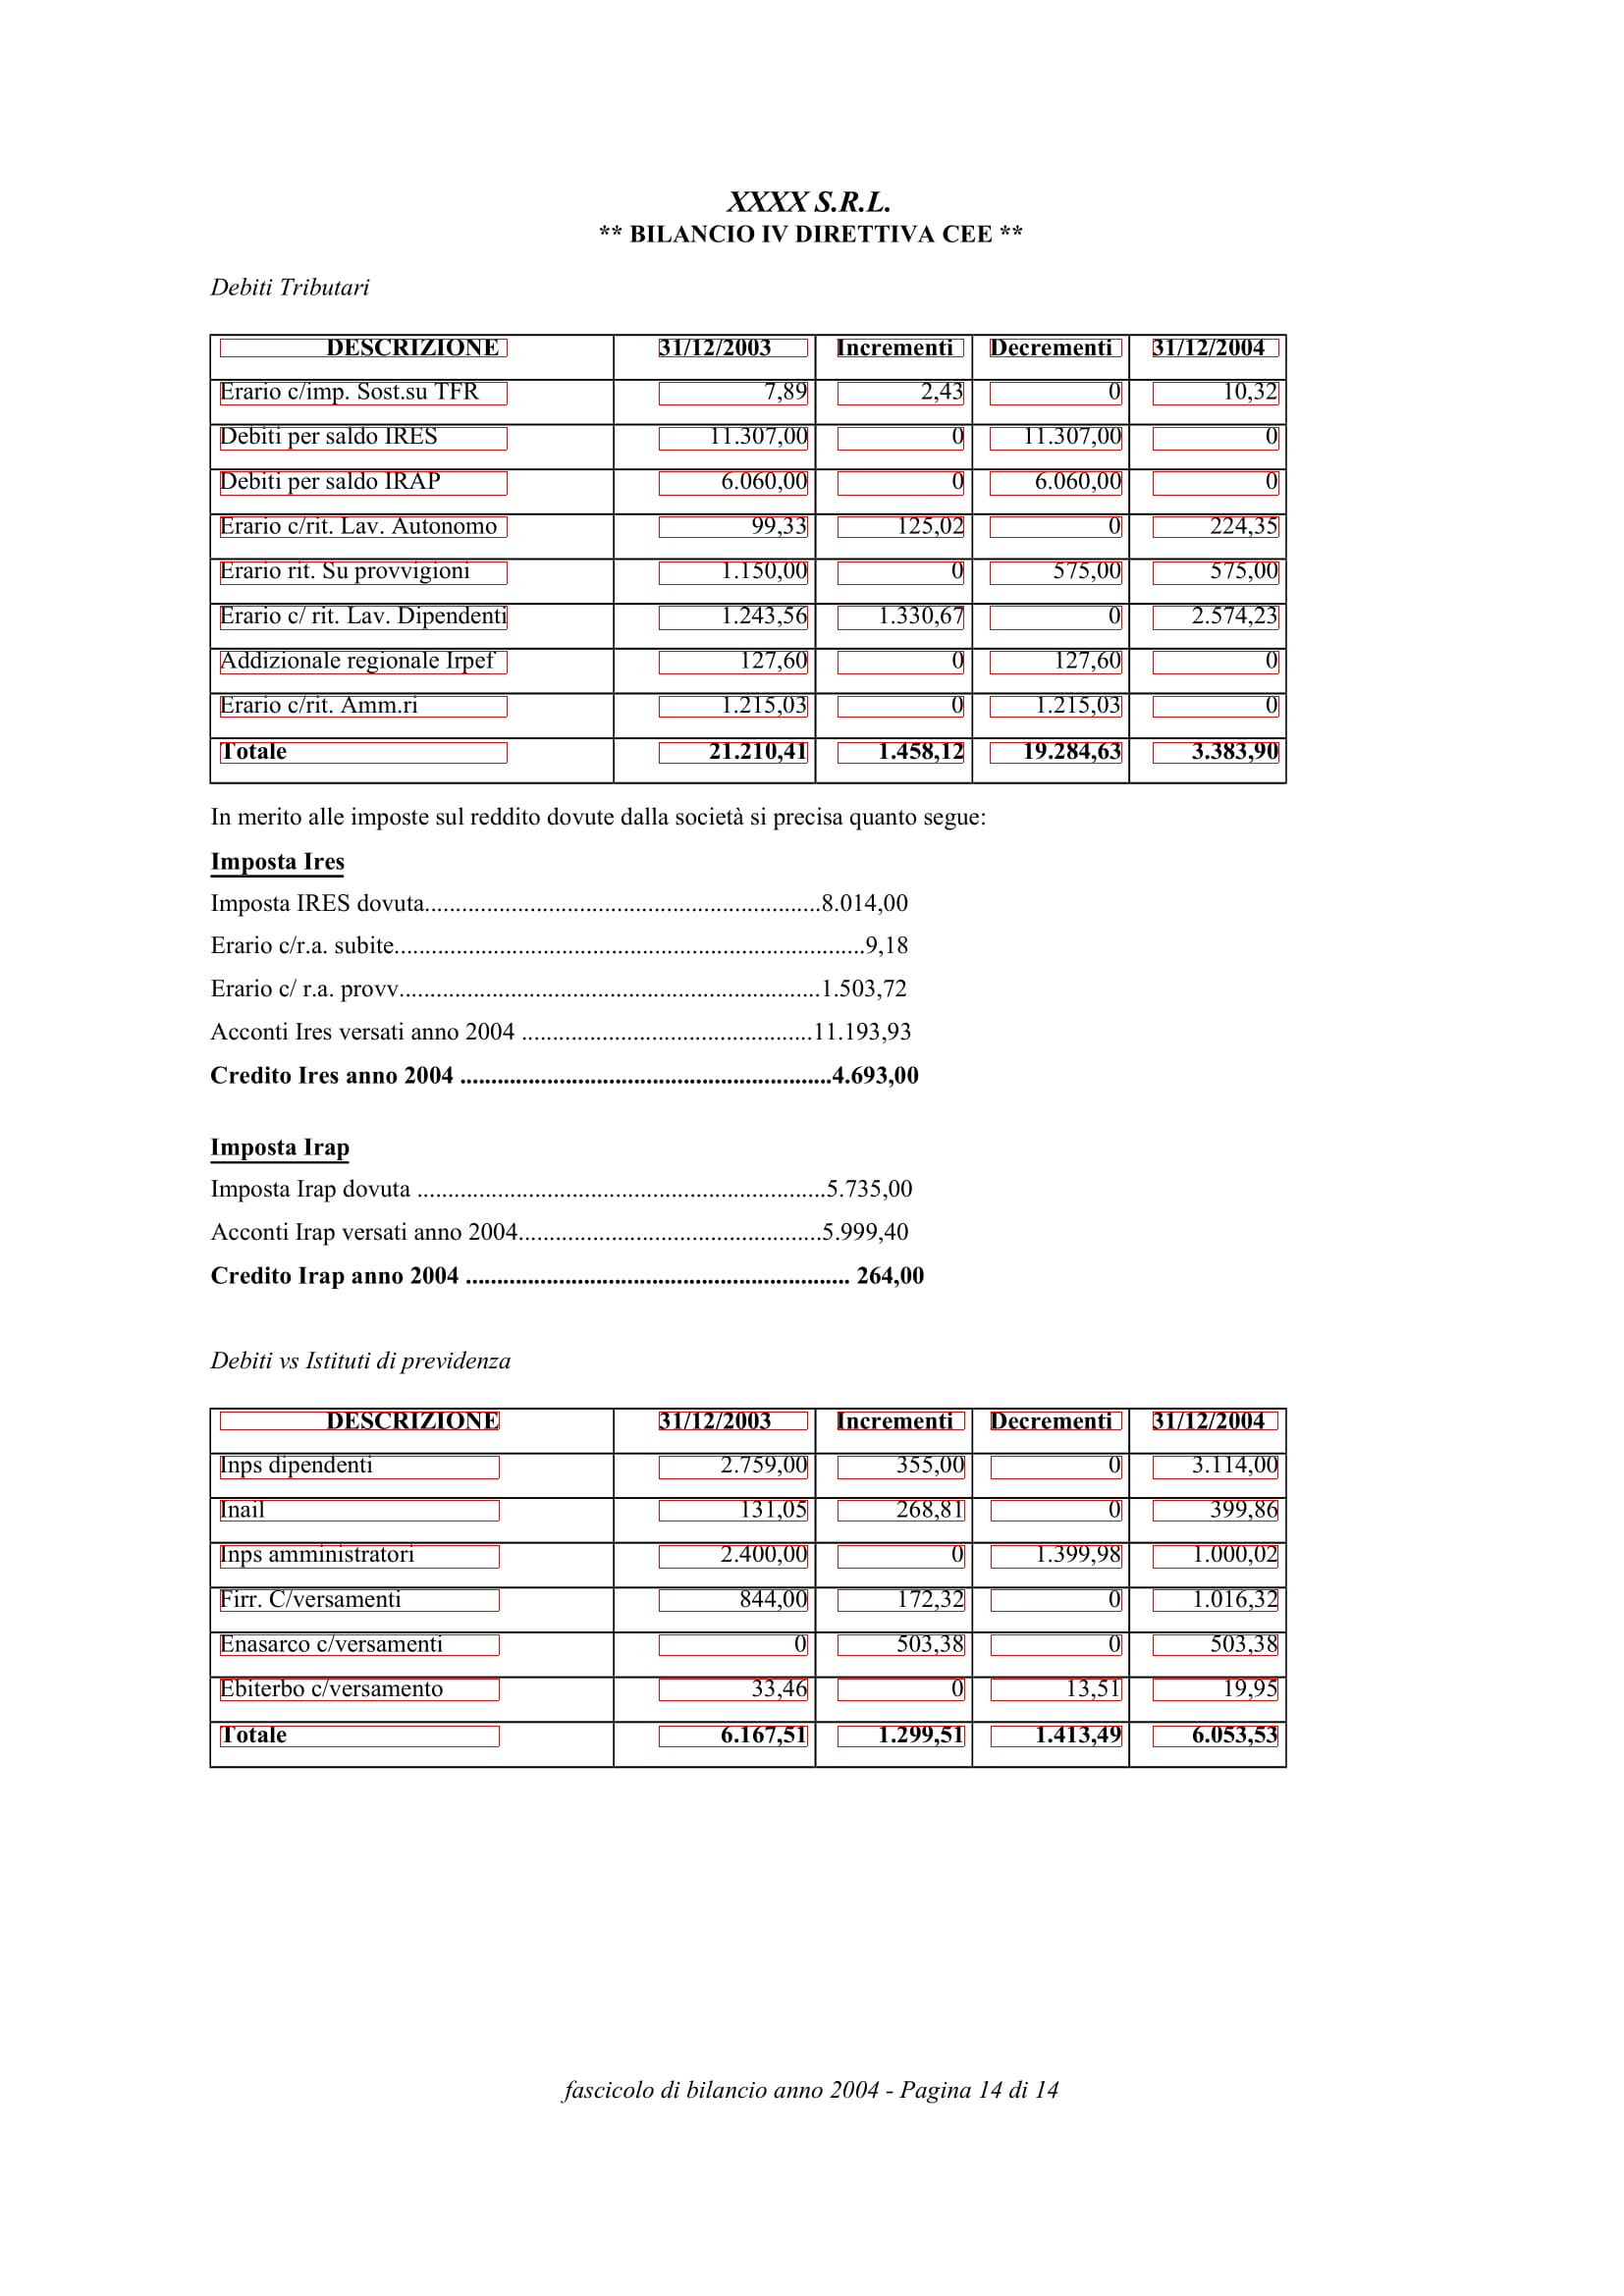
\includegraphics[width=15em]{img/results/goodRes1.png}
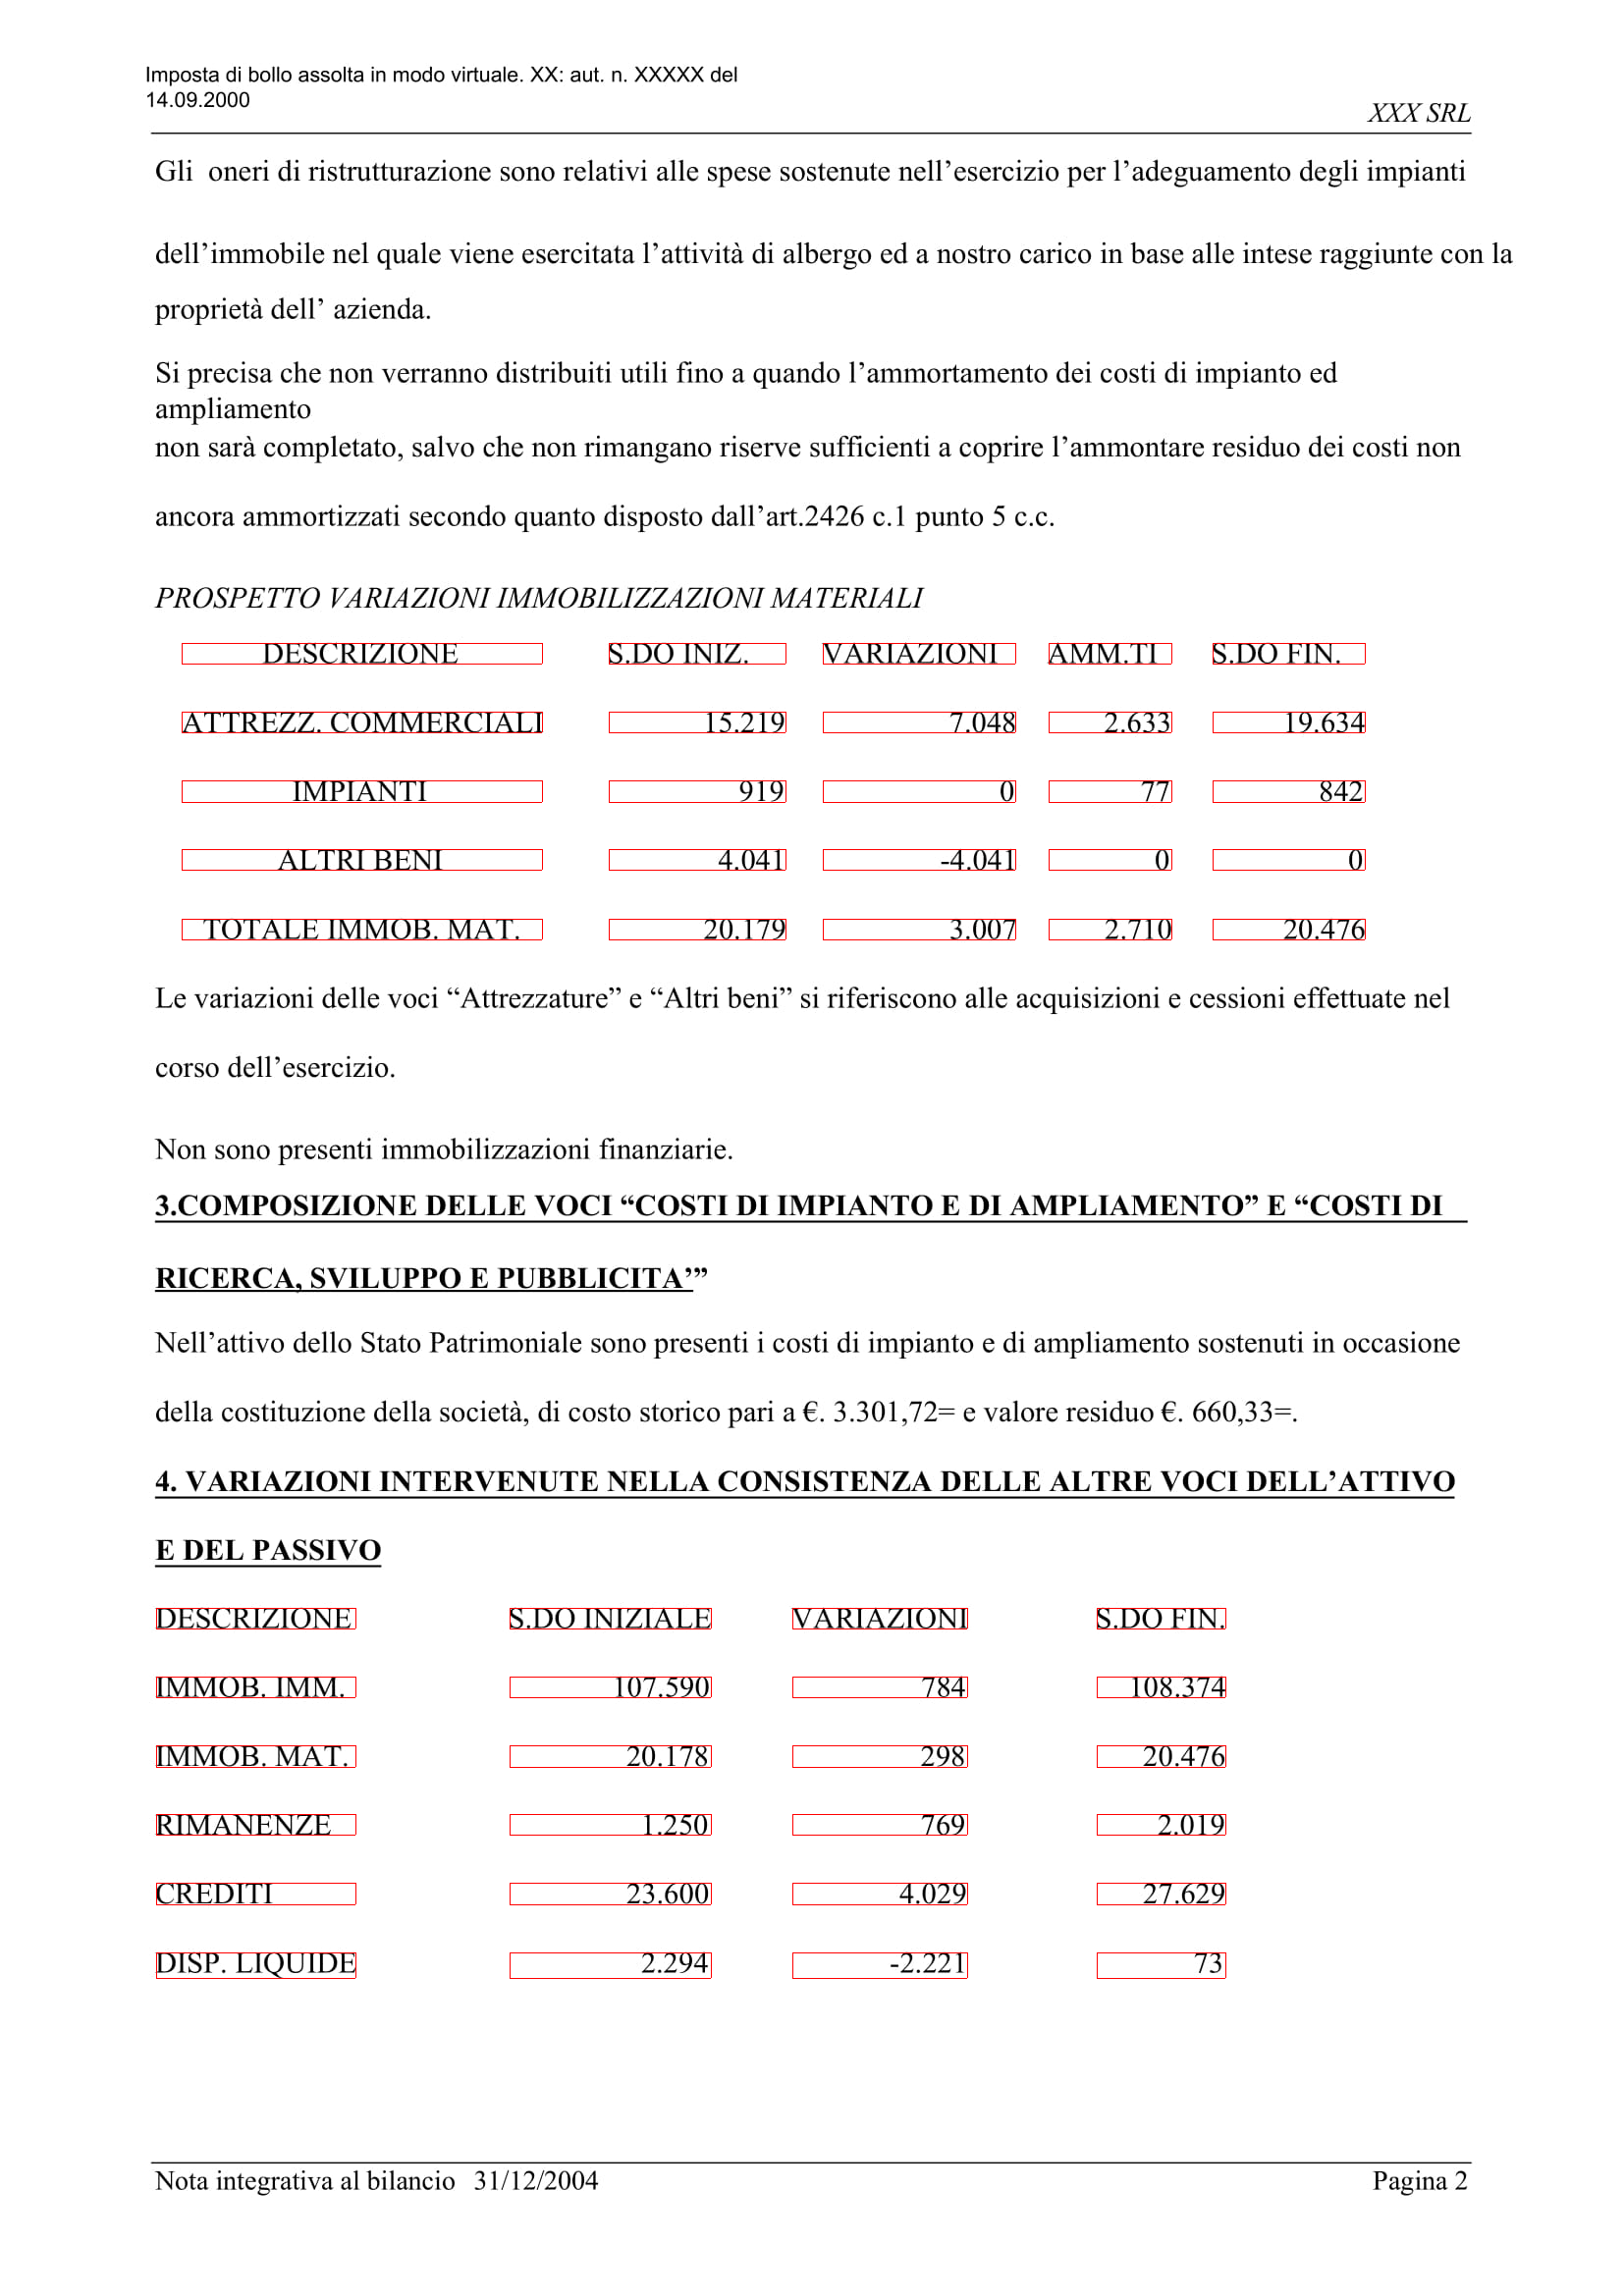
\includegraphics[width=15em]{img/results/goodRes2.png}
\caption{Correct table recognition (our implementation).}
\label{fig:sampleResults}
\end{figure}

\xxx{vsetky obrazky su na konci, preco?}